% Options for packages loaded elsewhere
% Options for packages loaded elsewhere
\PassOptionsToPackage{unicode}{hyperref}
\PassOptionsToPackage{hyphens}{url}
\PassOptionsToPackage{dvipsnames,svgnames,x11names}{xcolor}
%
\documentclass[
  spanish,
  11pt,
  letterpaper,
  DIV=11,
  numbers=noendperiod]{scrreprt}
\usepackage{xcolor}
\usepackage[margin=2.5cm]{geometry}
\usepackage{amsmath,amssymb}
\setcounter{secnumdepth}{5}
\usepackage{iftex}
\ifPDFTeX
  \usepackage[T1]{fontenc}
  \usepackage[utf8]{inputenc}
  \usepackage{textcomp} % provide euro and other symbols
\else % if luatex or xetex
  \usepackage{unicode-math} % this also loads fontspec
  \defaultfontfeatures{Scale=MatchLowercase}
  \defaultfontfeatures[\rmfamily]{Ligatures=TeX,Scale=1}
\fi
\usepackage{lmodern}
\ifPDFTeX\else
  % xetex/luatex font selection
\fi
% Use upquote if available, for straight quotes in verbatim environments
\IfFileExists{upquote.sty}{\usepackage{upquote}}{}
\IfFileExists{microtype.sty}{% use microtype if available
  \usepackage[]{microtype}
  \UseMicrotypeSet[protrusion]{basicmath} % disable protrusion for tt fonts
}{}
\makeatletter
\@ifundefined{KOMAClassName}{% if non-KOMA class
  \IfFileExists{parskip.sty}{%
    \usepackage{parskip}
  }{% else
    \setlength{\parindent}{0pt}
    \setlength{\parskip}{6pt plus 2pt minus 1pt}}
}{% if KOMA class
  \KOMAoptions{parskip=half}}
\makeatother
% Make \paragraph and \subparagraph free-standing
\makeatletter
\ifx\paragraph\undefined\else
  \let\oldparagraph\paragraph
  \renewcommand{\paragraph}{
    \@ifstar
      \xxxParagraphStar
      \xxxParagraphNoStar
  }
  \newcommand{\xxxParagraphStar}[1]{\oldparagraph*{#1}\mbox{}}
  \newcommand{\xxxParagraphNoStar}[1]{\oldparagraph{#1}\mbox{}}
\fi
\ifx\subparagraph\undefined\else
  \let\oldsubparagraph\subparagraph
  \renewcommand{\subparagraph}{
    \@ifstar
      \xxxSubParagraphStar
      \xxxSubParagraphNoStar
  }
  \newcommand{\xxxSubParagraphStar}[1]{\oldsubparagraph*{#1}\mbox{}}
  \newcommand{\xxxSubParagraphNoStar}[1]{\oldsubparagraph{#1}\mbox{}}
\fi
\makeatother


\usepackage{longtable,booktabs,array}
\newcounter{none} % for unnumbered tables
\usepackage{calc} % for calculating minipage widths
% Correct order of tables after \paragraph or \subparagraph
\usepackage{etoolbox}
\makeatletter
\patchcmd\longtable{\par}{\if@noskipsec\mbox{}\fi\par}{}{}
\makeatother
% Allow footnotes in longtable head/foot
\IfFileExists{footnotehyper.sty}{\usepackage{footnotehyper}}{\usepackage{footnote}}
\makesavenoteenv{longtable}
\usepackage{graphicx}
\makeatletter
\newsavebox\pandoc@box
\newcommand*\pandocbounded[1]{% scales image to fit in text height/width
  \sbox\pandoc@box{#1}%
  \Gscale@div\@tempa{\textheight}{\dimexpr\ht\pandoc@box+\dp\pandoc@box\relax}%
  \Gscale@div\@tempb{\linewidth}{\wd\pandoc@box}%
  \ifdim\@tempb\p@<\@tempa\p@\let\@tempa\@tempb\fi% select the smaller of both
  \ifdim\@tempa\p@<\p@\scalebox{\@tempa}{\usebox\pandoc@box}%
  \else\usebox{\pandoc@box}%
  \fi%
}
% Set default figure placement to htbp
\def\fps@figure{htbp}
\makeatother


% definitions for citeproc citations
\NewDocumentCommand\citeproctext{}{}
\NewDocumentCommand\citeproc{mm}{%
  \begingroup\def\citeproctext{#2}\cite{#1}\endgroup}
\makeatletter
 % allow citations to break across lines
 \let\@cite@ofmt\@firstofone
 % avoid brackets around text for \cite:
 \def\@biblabel#1{}
 \def\@cite#1#2{{#1\if@tempswa , #2\fi}}
\makeatother
\newlength{\cslhangindent}
\setlength{\cslhangindent}{1.5em}
\newlength{\csllabelwidth}
\setlength{\csllabelwidth}{3em}
\newenvironment{CSLReferences}[2] % #1 hanging-indent, #2 entry-spacing
 {\begin{list}{}{%
  \setlength{\itemindent}{0pt}
  \setlength{\leftmargin}{0pt}
  \setlength{\parsep}{0pt}
  % turn on hanging indent if param 1 is 1
  \ifodd #1
   \setlength{\leftmargin}{\cslhangindent}
   \setlength{\itemindent}{-1\cslhangindent}
  \fi
  % set entry spacing
  \setlength{\itemsep}{#2\baselineskip}}}
 {\end{list}}
\usepackage{calc}
\newcommand{\CSLBlock}[1]{\hfill\break\parbox[t]{\linewidth}{\strut\ignorespaces#1\strut}}
\newcommand{\CSLLeftMargin}[1]{\parbox[t]{\csllabelwidth}{\strut#1\strut}}
\newcommand{\CSLRightInline}[1]{\parbox[t]{\linewidth - \csllabelwidth}{\strut#1\strut}}
\newcommand{\CSLIndent}[1]{\hspace{\cslhangindent}#1}

\ifLuaTeX
\usepackage[bidi=basic,shorthands=off]{babel}
\else
\usepackage[bidi=default,shorthands=off]{babel}
\fi
\ifLuaTeX
  \usepackage{selnolig} % disable illegal ligatures
\fi


\setlength{\emergencystretch}{3em} % prevent overfull lines

\providecommand{\tightlist}{%
  \setlength{\itemsep}{0pt}\setlength{\parskip}{0pt}}



 


\usepackage{booktabs}
\usepackage{longtable}
\usepackage{array}
\usepackage{multirow}
\usepackage{wrapfig}
\usepackage{float}
\usepackage{colortbl}
\usepackage{pdflscape}
\usepackage{tabularx}
\usepackage{xltabular}
\usepackage{threeparttable}
\usepackage{threeparttablex}
\usepackage[normalem]{ulem}
\usepackage{makecell}
\usepackage{xcolor}
\KOMAoption{captions}{tableheading}
\makeatletter
\@ifpackageloaded{bookmark}{}{\usepackage{bookmark}}
\makeatother
\makeatletter
\@ifpackageloaded{caption}{}{\usepackage{caption}}
\AtBeginDocument{%
\ifdefined\contentsname
  \renewcommand*\contentsname{Tabla de contenidos}
\else
  \newcommand\contentsname{Tabla de contenidos}
\fi
\ifdefined\listfigurename
  \renewcommand*\listfigurename{Listado de Figuras}
\else
  \newcommand\listfigurename{Listado de Figuras}
\fi
\ifdefined\listtablename
  \renewcommand*\listtablename{Listado de Tablas}
\else
  \newcommand\listtablename{Listado de Tablas}
\fi
\ifdefined\figurename
  \renewcommand*\figurename{Figura}
\else
  \newcommand\figurename{Figura}
\fi
\ifdefined\tablename
  \renewcommand*\tablename{Tabla}
\else
  \newcommand\tablename{Tabla}
\fi
}
\@ifpackageloaded{float}{}{\usepackage{float}}
\floatstyle{ruled}
\@ifundefined{c@chapter}{\newfloat{codelisting}{h}{lop}}{\newfloat{codelisting}{h}{lop}[chapter]}
\floatname{codelisting}{Listado}
\newcommand*\listoflistings{\listof{codelisting}{Listado de Listados}}
\makeatother
\makeatletter
\makeatother
\makeatletter
\@ifpackageloaded{caption}{}{\usepackage{caption}}
\@ifpackageloaded{subcaption}{}{\usepackage{subcaption}}
\makeatother
\usepackage{bookmark}
\IfFileExists{xurl.sty}{\usepackage{xurl}}{} % add URL line breaks if available
\urlstyle{same}
% fallback for those not using the hyperref driver hyperxmp:
\makeatletter
\@ifundefined{xmpquote}{\newcommand{\xmpquote}[1]{#1}}{}
\makeatother
\hypersetup{
  pdftitle={Violencia basada en género},
  pdfauthor={José Ordoñez; Camila Gutiérrez; Marisol Vega},
  pdflang={es},
  colorlinks=true,
  linkcolor={blue},
  filecolor={Maroon},
  citecolor={Blue},
  urlcolor={Blue},
  pdfcreator={LaTeX via pandoc}}


\title{Violencia basada en género}
\author{José Ordoñez \and Camila Gutiérrez \and Marisol Vega}
\date{2025-12-31}
\begin{document}
\maketitle

\renewcommand*\contentsname{Tabla de contenidos}
{
\setcounter{tocdepth}{2}
\tableofcontents
}

\bookmarksetup{startatroot}

\chapter{Presentación}\label{presentaciuxf3n}

\section*{Sobre la investigación}\label{sobre-la-investigaciuxf3n}
\addcontentsline{toc}{section}{Sobre la investigación}

\markright{Sobre la investigación}

La presente investigación tiene como finalidad analizar las actitudes
frente a la violencia basada en género en los estudiantes de la
Universidad Nacional de Loja, considerando sus características
académicas, sociales y territoriales. Para ello, se utiliza una base de
datos proveniente de una encuesta estudiantil que contiene 1.452
registros, lo que permite desarrollar un diagnóstico sectorial y
territorial de las percepciones de los encuestados.

El estudio combina un análisis descriptivo con herramientas
estadísticas, como la prueba chi-cuadrado de independencia, para
examinar posibles asociaciones entre las actitudes frente a la violencia
basada en género y variables como el nivel de avance académico, el sexo
y la zona de origen. De esta manera, se busca aportar evidencia que
contribuya a comprender las percepciones estudiantiles y sirva como
referencia para fortalecer las estrategias de sensibilización y
prevención de la violencia basada en género en el ámbito universitario.

\section*{Autores}\label{autores}
\addcontentsline{toc}{section}{Autores}

\markright{Autores}

Camila Gutiérrez y Marisol Vega.

\bookmarksetup{startatroot}

\chapter{Introducción}\label{introducciuxf3n}

\section{Contextualización del
problema}\label{contextualizaciuxf3n-del-problema}

La violencia basada en género constituye una problemática social que
afecta las relaciones entre las personas y se encuentra vinculada con
factores culturales, educativos y sociales que pueden contribuir a su
aceptación, normalización o rechazo. Aunque en los últimos años se han
desarrollado iniciativas orientadas a promover la igualdad de género y
prevenir distintas manifestaciones de violencia, todavía persisten
creencias y comportamientos que dificultan su erradicación.

En el ámbito universitario, esta problemática adquiere especial
relevancia debido a que las instituciones de educación superior no solo
cumplen una función académica, sino que también constituyen espacios de
interacción social y formación de valores. Durante su trayectoria
universitaria, los estudiantes pueden adquirir conocimientos y
experiencias que influyan en sus percepciones sobre la igualdad, el
respeto y la violencia basada en género. Sin embargo, estas actitudes
también están condicionadas por experiencias personales, normas sociales
y características del entorno en el que se desarrollan.

En este contexto, resulta importante examinar las actitudes de los
estudiantes de la Universidad Nacional de Loja frente a la violencia
basada en género, considerando sus características sociodemográficas y
el nivel de avance académico. Este análisis permite comprender cómo se
distribuyen dichas actitudes dentro de la población encuestada y evaluar
si existen diferencias entre los estudiantes que se encuentran en
distintas etapas de su formación universitaria.

Por tanto, estudiar esta relación resulta pertinente para identificar
patrones de aceptación o rechazo hacia la violencia basada en género y
generar evidencia que contribuya a comprender esta problemática en el
entorno universitario, sin asumir que el avance académico constituye por
sí mismo un factor determinante de las actitudes estudiantiles.

\section{Planteamiento del problema}\label{planteamiento-del-problema}

A pesar de los avances en materia de igualdad de género y de las
iniciativas orientadas a prevenir la violencia basada en género, esta
problemática continúa presente en distintos espacios sociales, incluido
el ámbito universitario. Si bien la educación superior constituye un
espacio importante para la formación de conocimientos, valores y
actitudes, no necesariamente garantiza que todos los estudiantes
desarrollen las mismas percepciones frente a la violencia basada en
género.

En este contexto, resulta relevante analizar si el nivel de avance
académico de los estudiantes se relaciona con sus actitudes de
aceptación o rechazo hacia la violencia basada en género. A medida que
los estudiantes avanzan en su formación universitaria, pueden estar
expuestos a nuevas experiencias, conocimientos y espacios de reflexión
que contribuyan a modificar sus percepciones. Sin embargo, estas
actitudes también pueden estar relacionadas con factores personales,
familiares, sociales y culturales, por lo que no es posible atribuir sus
diferencias únicamente a la formación académica.

En la Universidad Nacional de Loja, la información obtenida mediante una
encuesta aplicada a 1.452 estudiantes permite examinar las actitudes
frente a la violencia basada en género y su relación con distintas
características sociodemográficas y académicas. No obstante, es
necesario determinar si existen diferencias estadísticamente
significativas entre los estudiantes de los niveles inicial, intermedio
y final de su formación universitaria.

Por ello, la presente investigación busca analizar la asociación entre
el nivel de avance académico y las actitudes frente a la violencia
basada en género, considerando además las características de la
población encuestada. Este análisis permitirá identificar patrones y
diferencias dentro del entorno universitario, aportando evidencia que
pueda contribuir a la comprensión de esta problemática y orientar
futuras estrategias de sensibilización y prevención.

\section{Pregunta de investigación}\label{pregunta-de-investigaciuxf3n}

¿Existe una asociación estadísticamente significativa entre el nivel de
avance académico y las actitudes frente a la violencia basada en género
en los estudiantes de la Universidad Nacional de Loja?

\section{Objetivo general}\label{objetivo-general}

Analizar la asociación entre el nivel de avance académico y las
actitudes frente a la violencia basada en género en los estudiantes de
la Universidad Nacional de Loja, mediante el análisis descriptivo y la
aplicación de pruebas estadísticas, considerando sus características
sociodemográficas y académicas.

\section{Objetivos específicos}\label{objetivos-especuxedficos}

\begin{itemize}
\item
  Caracterizar a la población estudiantil encuestada según sus
  condiciones sociodemográficas, académicas y socioeconómicas.
\item
  Describir la distribución de las actitudes frente a la violencia
  basada en género entre los estudiantes de la Universidad Nacional de
  Loja.
\item
  Examinar las diferencias en las actitudes frente a la violencia basada
  en género según los niveles inicial, intermedio y final de avance
  académico.
\item
  Evaluar la asociación estadística entre el nivel de avance académico y
  las actitudes frente a la violencia basada en género mediante la
  prueba de chi-cuadrado y el coeficiente V de Cramér.
\item
  Analizar la asociación entre las actitudes frente a la violencia
  basada en género y características sociodemográficas como el sexo y la
  zona de origen de los estudiantes.
\end{itemize}

\section{Justificación social e
institucional}\label{justificaciuxf3n-social-e-institucional}

La presente investigación se justifica por la importancia de comprender
las actitudes frente a la violencia basada en género dentro del ámbito
universitario, considerando que estas pueden reflejar la influencia de
normas sociales, experiencias personales y procesos de formación
académica. Analizar dichas actitudes permite reconocer diferencias entre
los estudiantes y aportar información relevante para la reflexión sobre
la prevención de la violencia y la promoción de relaciones basadas en el
respeto y la igualdad.

Desde una perspectiva social, el estudio contribuye a comprender cómo se
manifiestan las percepciones de aceptación o rechazo hacia la violencia
basada en género en una población estudiantil con diferentes
características sociodemográficas y académicas. Asimismo, permite
examinar si el avance en la formación universitaria presenta alguna
asociación con estas actitudes, reconociendo que pueden intervenir otros
factores que no necesariamente se encuentran determinados por el nivel
educativo.

Desde el ámbito institucional, la investigación proporciona información
sobre las características y percepciones de los estudiantes de la
Universidad Nacional de Loja. Los resultados pueden servir como
referencia para orientar futuras actividades de sensibilización,
prevención y formación relacionadas con la violencia basada en género,
considerando las particularidades de la población universitaria.

Finalmente, el estudio tiene relevancia académica porque utiliza
información cuantitativa y herramientas estadísticas para examinar la
relación entre el avance académico y las actitudes estudiantiles,
contribuyendo a la generación de evidencia que puede servir como punto
de partida para investigaciones posteriores.

\section{Alcance}\label{alcance}

La investigación se desarrolla a partir de una encuesta aplicada a 1.452
estudiantes de la Universidad Nacional de Loja, con el propósito de
analizar sus actitudes frente a la violencia basada en género y su
asociación con el nivel de avance académico. El estudio considera
características sociodemográficas, académicas y socioeconómicas, entre
ellas el sexo, la edad, la facultad, la situación laboral, la clase
social autopercibida y la zona de origen.

El análisis tiene un alcance descriptivo y asociativo. En primer lugar,
se caracteriza a la población encuestada mediante distribuciones de
frecuencias, porcentajes y representaciones gráficas. Posteriormente, se
examina la relación entre el nivel de avance académico y las actitudes
frente a la violencia basada en género mediante pruebas estadísticas de
asociación. También se consideran las diferencias relacionadas con el
sexo y la zona de origen de los estudiantes.

Es importante señalar que, debido al carácter transversal de la
información, los resultados permiten identificar asociaciones
estadísticas, pero no establecer relaciones causales ni determinar que
el avance académico produce cambios en las actitudes frente a la
violencia basada en género. Asimismo, los hallazgos corresponden a la
población estudiada y no deben generalizarse automáticamente a otras
instituciones de educación superior.

De esta manera, la investigación busca aportar evidencia sobre las
actitudes estudiantiles frente a la violencia basada en género y su
relación con determinadas características académicas y
sociodemográficas, ofreciendo información que puede contribuir a futuras
investigaciones y estrategias institucionales de prevención.

\bookmarksetup{startatroot}

\chapter{Datos y variables}\label{datos-y-variables}

\section{Fuente de información}\label{fuente-de-informaciuxf3n}

La presente investigación utiliza microdatos provenientes de una
encuesta aplicada a estudiantes de la Universidad Nacional de Loja
(UNL), orientada a recopilar información sobre sus características
sociodemográficas, académicas y sus actitudes frente a la violencia
basada en género.

La base de datos original contiene 1.452 registros y 122 variables, que
permiten caracterizar a la población encuestada y examinar posibles
asociaciones entre las actitudes frente a la violencia basada en género
y determinadas características de los estudiantes. Para el desarrollo
del estudio se seleccionaron las variables relacionadas con el nivel de
avance académico, el sexo, la edad, la facultad, la situación laboral,
la clase social autopercibida y la procedencia territorial.

La información constituye una fuente de datos de corte transversal, por
lo que permite analizar las características y asociaciones observadas
entre las variables, sin establecer relaciones causales ni evaluar
cambios individuales a lo largo del tiempo.

\section{Variables principales}\label{variables-principales}

\begingroup\fontsize{9}{11}\selectfont

\begin{longtable}[t]{llcl}

\caption{\label{tbl-variables}Descripción de las variables del estudio}

\tabularnewline

\toprule
\textbf{Tipo de variable} & \textbf{Variable} & \textbf{Código} & \textbf{Descripción}\\
\midrule
Dependiente & Rechazo de la VBG & VBG\_INACEPT\_B1\_5 & Percepción sobre si la violencia basada en género es inaceptable.\\
Independiente & Nivel de avance académico & NIVEL\_SEMSTRE & Clasificación del estudiante en nivel inicial, intermedio o final.\\
Control & Edad & EDAD & Edad de la persona encuestada.\\
Control & Sexo & SEXO\_13 & Sexo declarado por la persona encuestada.\\
Control & Situación laboral & TRAB\_EST\_9 & Condición de estudio y trabajo.\\
\addlinespace
Control & Clase social & CLASE\_SOCIAL\_17 & Clase social autopercibida.\\
Control & Facultad & FACULTAD\_4 & Facultad o área académica a la que pertenece.\\
\bottomrule

\end{longtable}

\endgroup{}

\section{Construcción de
indicadores}\label{construcciuxf3n-de-indicadores}

Para el desarrollo de la investigación se consideran dos variables
principales: las actitudes frente a la violencia basada en género y el
nivel de avance académico de los estudiantes.

La variable correspondiente a las actitudes frente a la violencia basada
en género se obtiene mediante el ítem VBG\_INACEPT\_B1\_5, que recoge
las respuestas de los estudiantes ante la afirmación «La violencia
basada en género es inaceptable». Este indicador presenta cinco
categorías de respuesta, donde la categoría 5 representa el mayor grado
de acuerdo con la afirmación. Por tanto, las respuestas permiten
identificar diferentes niveles de aceptación o rechazo hacia la
violencia basada en género.

Por otra parte, el nivel de avance académico se identifica mediante la
variable NIVEL\_SEMESTRE, agrupada en tres categorías: inicial,
intermedio y final. Esta clasificación permite comparar las actitudes de
los estudiantes según la etapa de formación universitaria en la que se
encuentran.

Adicionalmente, se incorporan variables sociodemográficas y
socioeconómicas, como el sexo, la edad, la situación laboral, la clase
social autopercibida, la facultad y la zona de origen, con el propósito
de caracterizar a la población encuestada y complementar el análisis de
las diferencias observadas entre los estudiantes.

{\def\LTcaptype{none} % do not increment counter
\begin{longtable}[]{@{}
  >{\raggedright\arraybackslash}p{(\linewidth - 6\tabcolsep) * \real{0.2737}}
  >{\raggedright\arraybackslash}p{(\linewidth - 6\tabcolsep) * \real{0.1789}}
  >{\raggedright\arraybackslash}p{(\linewidth - 6\tabcolsep) * \real{0.3158}}
  >{\raggedleft\arraybackslash}p{(\linewidth - 6\tabcolsep) * \real{0.2316}}@{}}
\toprule\noalign{}
\begin{minipage}[b]{\linewidth}\raggedright
Indicador
\end{minipage} & \begin{minipage}[b]{\linewidth}\raggedright
Código
\end{minipage} & \begin{minipage}[b]{\linewidth}\raggedright
Categorías
\end{minipage} & \begin{minipage}[b]{\linewidth}\raggedleft
Observaciones válidas
\end{minipage} \\
\midrule\noalign{}
\endhead
\bottomrule\noalign{}
\endlastfoot
Actitud frente a la VBG & VBG\_INACEPT\_B1\_5 & Cinco categorías de
respuesta & 1452 \\
Nivel de avance académico & NIVEL\_SEMSTRE & Inicial, intermedio y final
& 1442 \\
\end{longtable}
}

\section{Tratamiento de datos}\label{tratamiento-de-datos}

La base de datos original contiene 1.452 registros correspondientes a
estudiantes encuestados de la Universidad Nacional de Loja. Como parte
del tratamiento de la información, se revisó la disponibilidad de las
variables seleccionadas y la presencia de valores faltantes.

La revisión permitió identificar que la variable correspondiente a las
actitudes frente a la violencia basada en género cuenta con 1.452
observaciones válidas, mientras que el nivel de avance académico
presenta 1.442 observaciones válidas y 10 registros sin información
disponible.

En consecuencia, para el análisis de asociación entre el nivel de avance
académico y las actitudes frente a la violencia basada en género se
utilizaron 1.442 observaciones con información disponible en ambas
variables. Esta selección permite realizar las comparaciones
estadísticas correspondientes sin incorporar registros incompletos en
las variables principales del análisis.

Posteriormente, se desarrolló un análisis descriptivo mediante tablas de
frecuencias, porcentajes y representaciones gráficas. Para examinar la
asociación entre las variables categóricas se aplicaron pruebas
estadísticas de chi-cuadrado y se utilizó el coeficiente V de Cramér
para evaluar la intensidad de la asociación observada.

{\def\LTcaptype{none} % do not increment counter
\begin{longtable}[]{@{}lc@{}}
\toprule\noalign{}
Indicador & Observaciones \\
\midrule\noalign{}
\endhead
\bottomrule\noalign{}
\endlastfoot
Registros originales & 1452 \\
Valores faltantes en variable dependiente & 0 \\
Valores faltantes en variable independiente & 10 \\
Valores faltantes en edad & 0 \\
Valores faltantes en sexo & 0 \\
Valores faltantes en situación laboral & 0 \\
Valores faltantes en clase social & 0 \\
Valores faltantes en facultad & 0 \\
\end{longtable}
}

\section{Alcance de la información}\label{alcance-de-la-informaciuxf3n}

La información utilizada permite caracterizar a los estudiantes
encuestados de la Universidad Nacional de Loja y examinar la asociación
entre el nivel de avance académico y las actitudes frente a la violencia
basada en género. Asimismo, facilita la identificación de diferencias
descriptivas según características sociodemográficas, académicas y
territoriales.

No obstante, los resultados deben interpretarse considerando las
limitaciones de la información disponible. Al tratarse de datos
transversales, no es posible determinar si las actitudes de los
estudiantes cambian como consecuencia de su avance académico, puesto que
no se realiza un seguimiento de los mismos individuos a lo largo del
tiempo.

Además, las actitudes analizadas corresponden a respuestas declaradas
por los participantes ante una afirmación específica, por lo que no
representan necesariamente sus comportamientos reales frente a
situaciones de violencia basada en género.

Por tanto, los resultados permiten identificar patrones y asociaciones
dentro de la población encuestada, pero no establecer relaciones
causales ni generalizar automáticamente los hallazgos a toda la
población universitaria del país.

\bookmarksetup{startatroot}

\chapter{Diagnóstico sectorial}\label{diagnuxf3stico-sectorial}

\section{Caracterización de la población
encuestada}\label{caracterizaciuxf3n-de-la-poblaciuxf3n-encuestada}

El diagnóstico sectorial tiene como finalidad describir las principales
características sociodemográficas y académicas de las personas
encuestadas en la Universidad Nacional de Loja, así como examinar sus
percepciones frente a la violencia basada en género. Para ello, se
utiliza una base de datos que contiene 1.452 registros y 122 variables,
de las cuales se seleccionaron aquellas relacionadas con el sexo, la
edad, la situación laboral, la clase social, la facultad, el nivel de
avance académico y las actitudes frente a la violencia basada en género.

A partir de esta información, se realiza un análisis descriptivo
mediante tablas de frecuencias, porcentajes y representaciones gráficas,
con el propósito de identificar las características predominantes de la
población encuestada y explorar posibles diferencias en sus
percepciones. Este diagnóstico constituye una base para comprender cómo
se distribuyen las actitudes frente a la violencia basada en género
entre los distintos grupos de estudiantes, sin establecer relaciones de
causalidad.

\section{Distribución de la población encuestada por sexo y
edad}\label{distribuciuxf3n-de-la-poblaciuxf3n-encuestada-por-sexo-y-edad}

El análisis de las características sociodemográficas de la población
encuestada permite conocer la composición de los participantes y
establecer un contexto para el estudio de las actitudes frente a la
violencia basada en género. En este sentido, se consideran dos variables
fundamentales: el sexo y la edad, debido a que ambas permiten
identificar diferencias en la estructura de la población universitaria y
posteriormente explorar posibles variaciones en las percepciones de los
estudiantes.

A partir de la información recopilada en la Universidad Nacional de
Loja, se examina la distribución de los participantes según el sexo
declarado y los grupos de edad. Para ello, se utilizan frecuencias
absolutas y relativas, acompañadas de representaciones gráficas que
facilitan la interpretación de los resultados.

\begin{figure}

\centering{

\pandocbounded{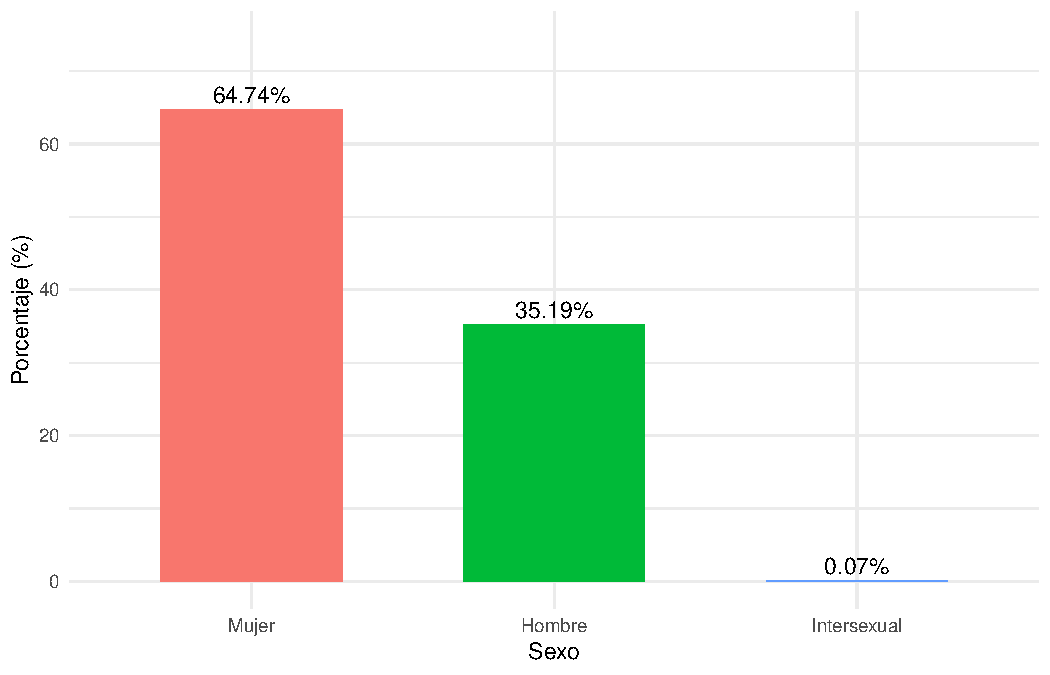
\includegraphics[keepaspectratio]{capitulos/Diagnóstico-sectorial_files/figure-pdf/fig-distribucion-sexo-1.pdf}}

}

\caption{\label{fig-distribucion-sexo}Distribución porcentual de la
población encuestada según sexo}

\end{figure}%

Los resultados muestran una mayor participación de mujeres (64,74 \%),
seguidas de los hombres (35,19 \%) y las personas intersexuales (0,07
\%). Esta diferencia evidencia una mayor representación femenina en la
muestra, aspecto importante al analizar las percepciones sobre la
violencia basada en género, aunque no permite establecer diferencias en
las actitudes de rechazo sin comparar las respuestas de cada grupo.

\begin{figure}

\centering{

\pandocbounded{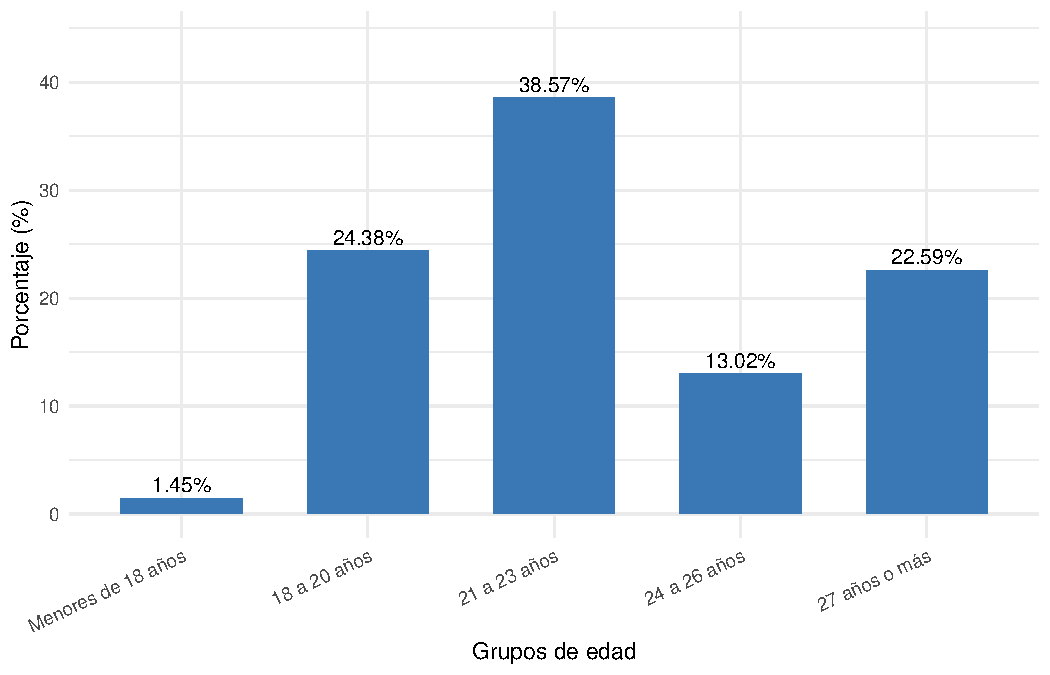
\includegraphics[keepaspectratio]{capitulos/Diagnóstico-sectorial_files/figure-pdf/fig-grupos-edad-1.pdf}}

}

\caption{\label{fig-grupos-edad}Distribución porcentual de los
encuestados por grupos de edad}

\end{figure}%

Los resultados muestran que la mayor proporción de encuestados se
concentra entre los 21 y 23 años (38,57 \%), seguida del grupo de 18 a
20 años (24,38 \%) y de 27 años o más (22,59 \%). En menor proporción se
encuentran los estudiantes de 24 a 26 años (13,02 \%) y los menores de
18 años (1,45 \%). Esto evidencia que la muestra está conformada
principalmente por jóvenes universitarios, aspecto relevante para
analizar sus percepciones frente a la violencia basada en género.

\section{Características académicas de la población
encuestada}\label{caracteruxedsticas-acaduxe9micas-de-la-poblaciuxf3n-encuestada}

El análisis de las características académicas permite identificar cómo
se distribuyen los estudiantes encuestados según la facultad a la que
pertenecen y su nivel de avance en la formación universitaria. Estas
variables son relevantes para la investigación, ya que permiten conocer
la composición académica de la muestra y posteriormente examinar
posibles diferencias en las actitudes frente a la violencia basada en
género, considerando las distintas etapas de formación de los
estudiantes.

\begin{figure}

\centering{

\pandocbounded{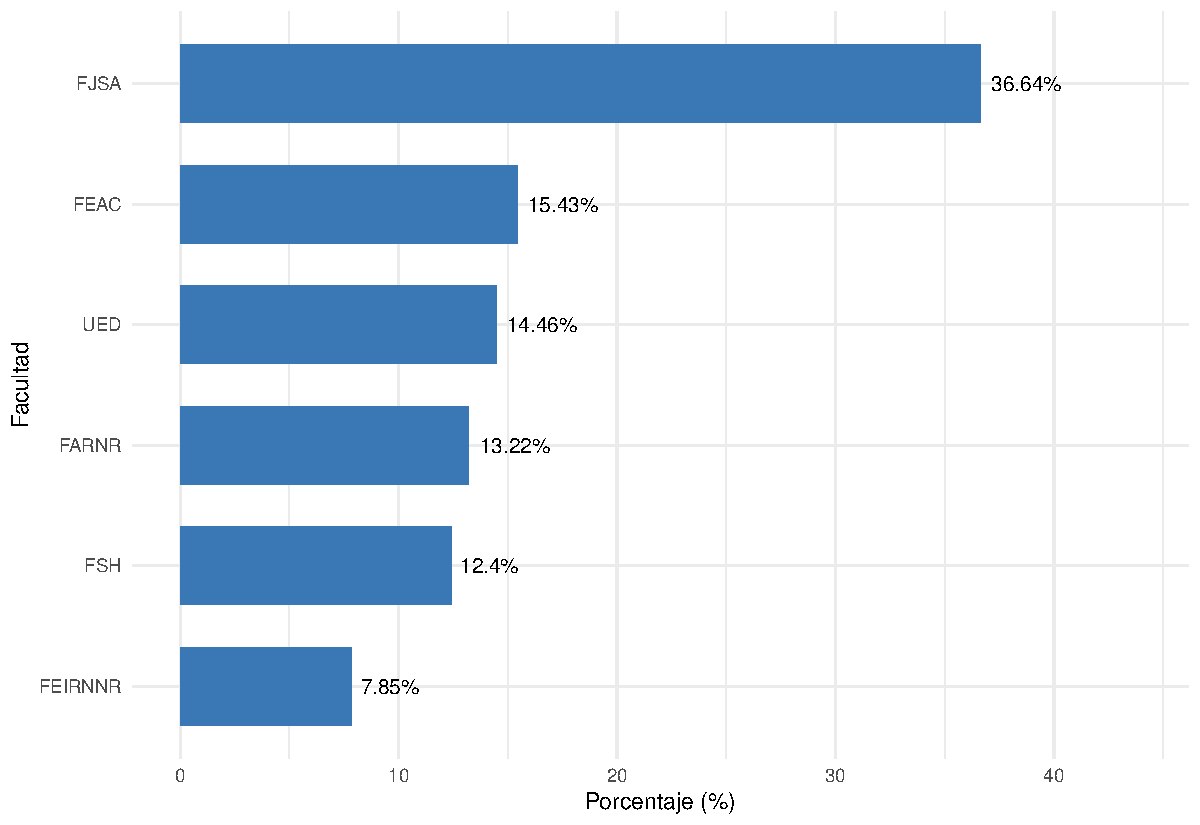
\includegraphics[keepaspectratio]{capitulos/Diagnóstico-sectorial_files/figure-pdf/fig-distribucion-facultad-1.pdf}}

}

\caption{\label{fig-distribucion-facultad}Distribución porcentual de los
encuestados según facultad}

\end{figure}%

Los resultados muestran que la mayor proporción de encuestados pertenece
a la facultad FJSA (36,64 \%), seguida de FEAC (15,43 \%) y UED (14,46
\%). Por su parte, FARNR (13,22 \%) y FSH (12,40 \%) presentan una
participación intermedia, mientras que FEIRNNR registra el menor
porcentaje (7,85 \%). Esta distribución evidencia una participación
desigual entre las facultades, aspecto importante al analizar las
percepciones sobre la violencia basada en género, debido a que algunas
áreas académicas tienen mayor representación en la muestra.

\begin{figure}

\centering{

\pandocbounded{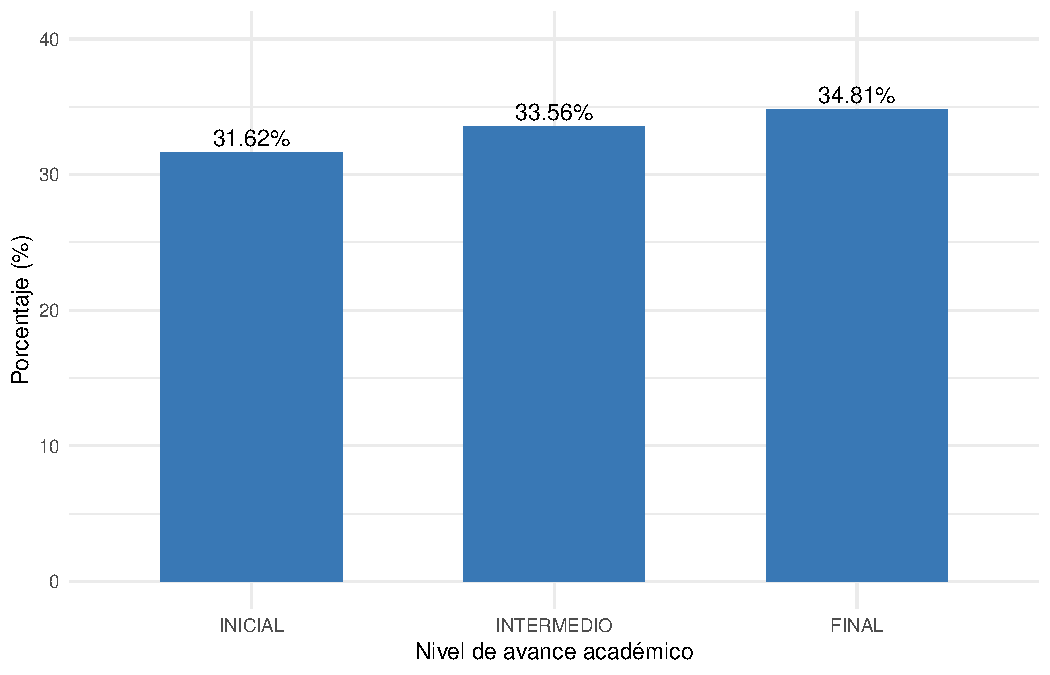
\includegraphics[keepaspectratio]{capitulos/Diagnóstico-sectorial_files/figure-pdf/fig-nivel-academico-1.pdf}}

}

\caption{\label{fig-nivel-academico}Distribución porcentual según nivel
de avance académico}

\end{figure}%

Los resultados muestran una distribución relativamente equilibrada de
los estudiantes según su nivel de avance académico, con una mayor
participación del nivel final (34,81 \%), seguido del intermedio (33,56
\%) y el inicial (31,62 \%). Estas diferencias son reducidas, lo que
permite contar con una representación similar de los tres grupos y
facilita la comparación de sus percepciones frente a la violencia basada
en género a lo largo de su formación universitaria.

\subsection{Condiciones socioeconómicas de la población
encuestada}\label{condiciones-socioeconuxf3micas-de-la-poblaciuxf3n-encuestada}

El análisis de las condiciones socioeconómicas permite conocer la
situación laboral y la clase social autopercibida de los estudiantes
encuestados. Estas características son relevantes para contextualizar
las diferencias económicas y sociales presentes en la población
universitaria y posteriormente examinar su posible relación con las
actitudes frente a la violencia basada en género.

\begin{figure}

\centering{

\pandocbounded{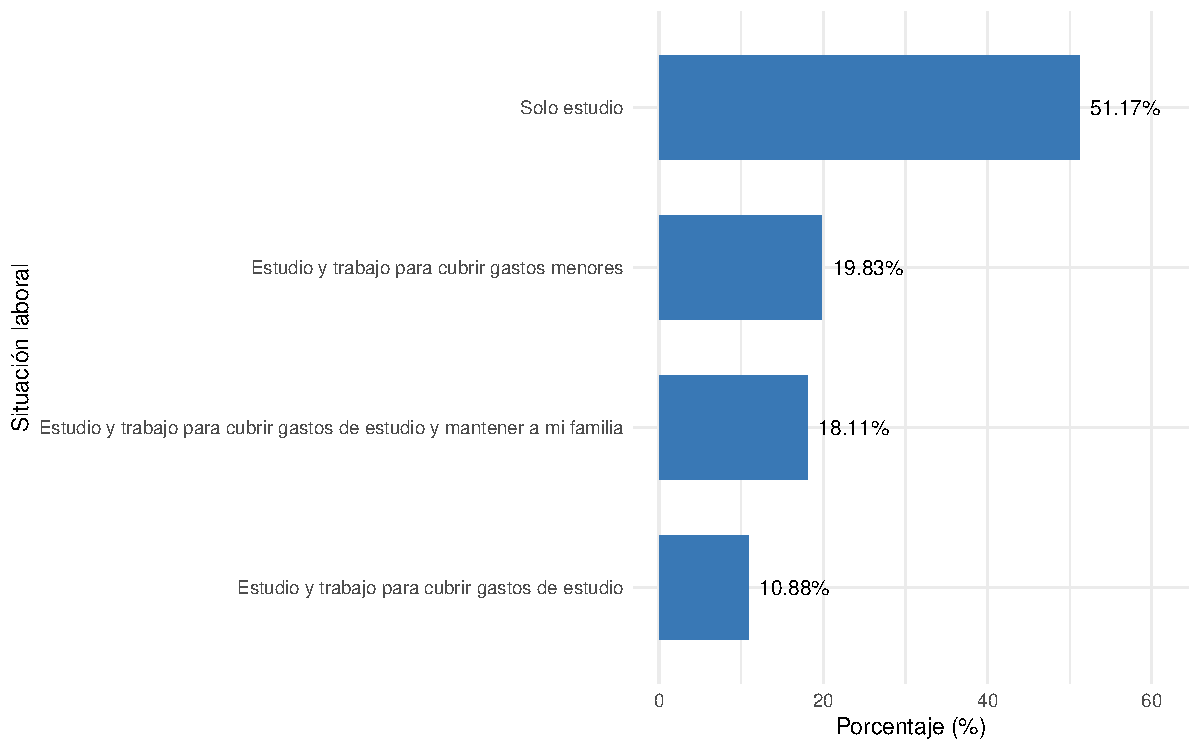
\includegraphics[keepaspectratio]{capitulos/Diagnóstico-sectorial_files/figure-pdf/fig-situacion-laboral-1.pdf}}

}

\caption{\label{fig-situacion-laboral}Distribución porcentual según
situación laboral}

\end{figure}%

Los resultados muestran que el 51,17 \% de los encuestados se dedica
únicamente a estudiar, mientras que el 19,83 \% estudia y trabaja para
cubrir gastos menores. Por otro lado, el 18,11 \% combina sus estudios
con el trabajo para financiar su educación y mantener a su familia, y el
10,88 \% trabaja para cubrir gastos académicos. Esto evidencia que,
aunque predomina la dedicación exclusiva al estudio, una proporción
importante de estudiantes enfrenta responsabilidades económicas
adicionales, lo que refleja distintas condiciones socioeconómicas dentro
de la población universitaria.

\begin{figure}

\centering{

\pandocbounded{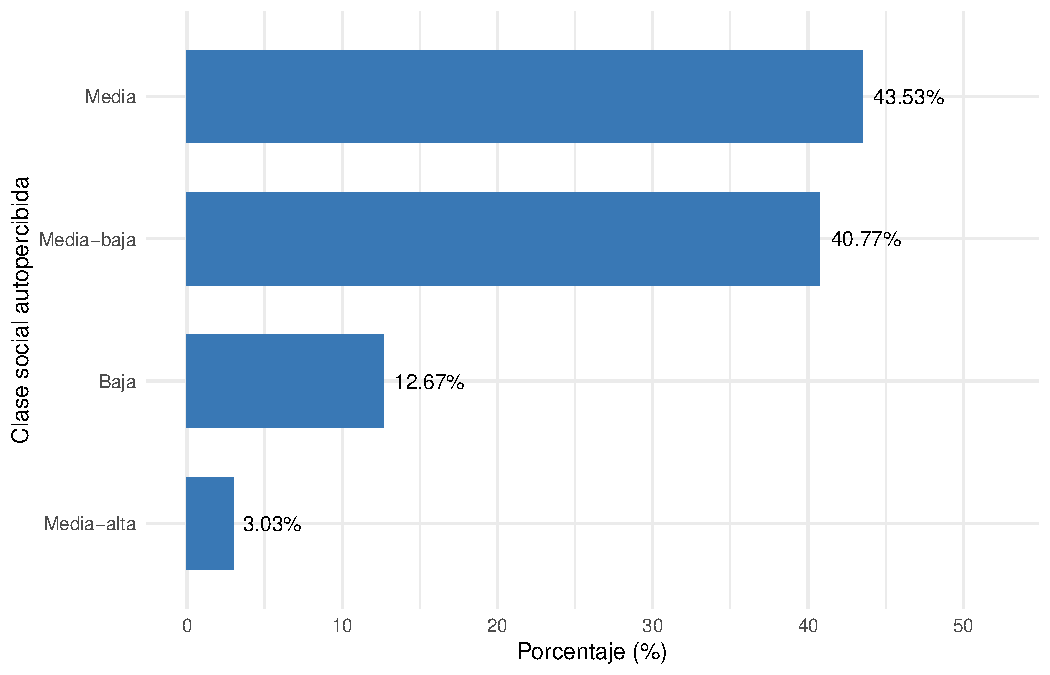
\includegraphics[keepaspectratio]{capitulos/Diagnóstico-sectorial_files/figure-pdf/fig-clase-social-1.pdf}}

}

\caption{\label{fig-clase-social}Distribución porcentual según clase
social autopercibida}

\end{figure}%

Los resultados muestran que la mayoría de los encuestados se identifica
con la clase media (43,53 \%), seguida de la clase media-baja (40,77
\%). En menor proporción se encuentran quienes se consideran de clase
baja (12,67 \%) y media-alta (3,03 \%). Esto evidencia que predominan
los estudiantes que se perciben dentro de los estratos medios y
medios-bajos, lo que refleja diferencias en las condiciones
socioeconómicas de la población universitaria y constituye un aspecto
relevante para analizar sus percepciones frente a la violencia basada en
género.

\section{Actitudes frente a la violencia basada en
género}\label{actitudes-frente-a-la-violencia-basada-en-guxe9nero}

El análisis de las actitudes frente a la violencia basada en género
permite conocer las percepciones de los estudiantes de la Universidad
Nacional de Loja respecto al rechazo de estas conductas. Para ello, se
utiliza la variable la violencia basada en género es inaceptable, que
recoge cinco categorías de respuesta. Su distribución permite
identificar las posturas predominantes entre los encuestados y
constituye un punto de partida para examinar posteriormente las
diferencias según el nivel de avance académico y las características
sociodemográficas.

\begin{figure}

\centering{

\pandocbounded{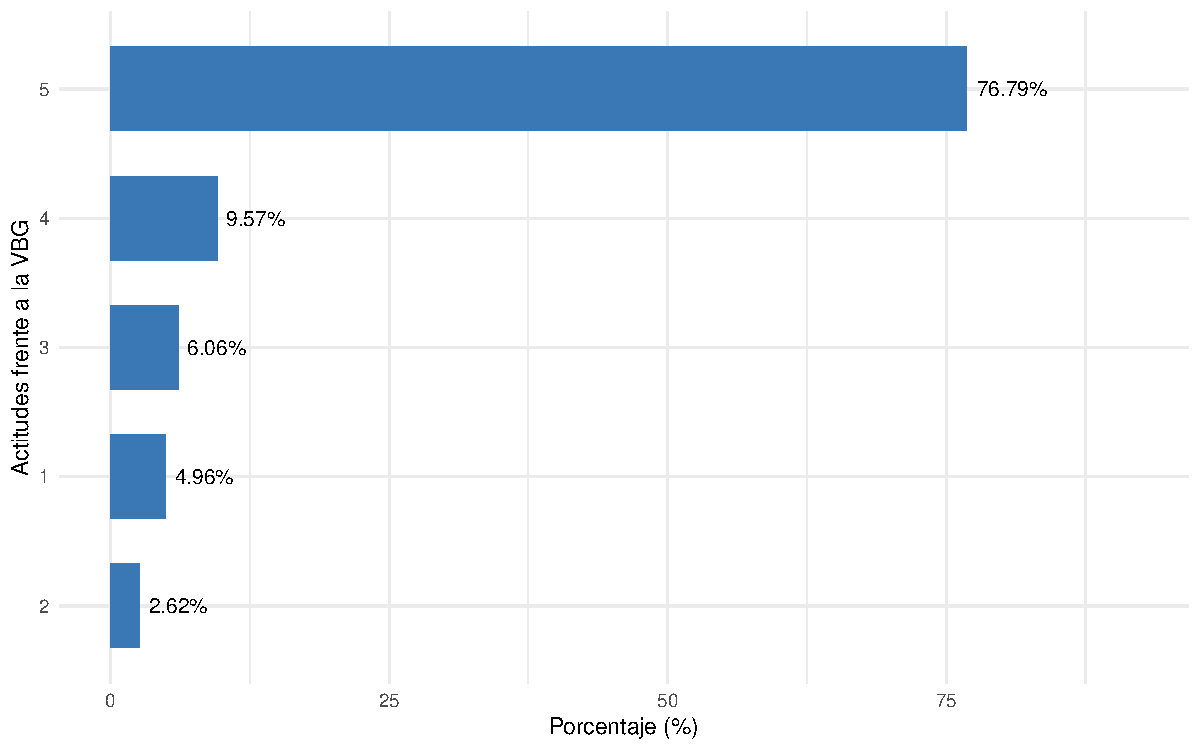
\includegraphics[keepaspectratio]{capitulos/Diagnóstico-sectorial_files/figure-pdf/fig-actitudes-vbg-1.pdf}}

}

\caption{\label{fig-actitudes-vbg}Distribución porcentual de las
actitudes frente a la violencia basada en género}

\end{figure}%

Los resultados muestran que el 76,79 \% de los encuestados seleccionó la
categoría 5 respecto a la afirmación «La violencia basada en género es
inaceptable», seguido del 9,57 \% en la categoría 4. En contraste, las
categorías 1, 2 y 3 presentan porcentajes menores. Esto evidencia una
marcada concentración de respuestas en los valores superiores de la
escala, lo que podría reflejar una actitud de rechazo hacia la violencia
basada en género, siempre que estos valores representen un mayor grado
de acuerdo con la afirmación.

\section{Actitudes frente a la violencia basada en género según el nivel
de avance
académico}\label{actitudes-frente-a-la-violencia-basada-en-guxe9nero-seguxfan-el-nivel-de-avance-acaduxe9mico}

El análisis de las actitudes frente a la violencia basada en género
según el nivel de avance académico permite identificar posibles
diferencias en las percepciones de los estudiantes a lo largo de su
formación universitaria. Para ello, se comparan las respuestas de los
estudiantes de nivel inicial, intermedio y final respecto a la
afirmación «La violencia basada en género es inaceptable», con el
propósito de determinar si existen variaciones en el grado de acuerdo
entre los distintos grupos académicos.

\begin{figure}

\centering{

\pandocbounded{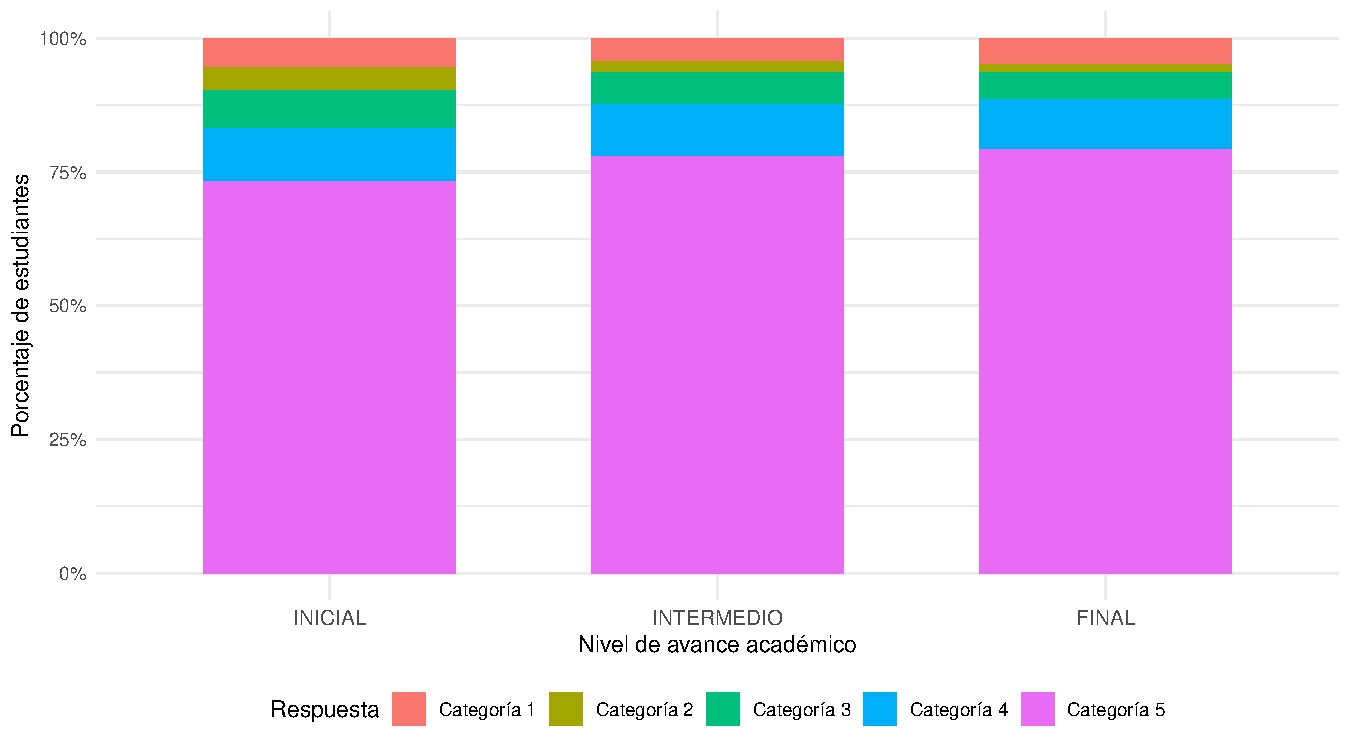
\includegraphics[keepaspectratio]{capitulos/Diagnóstico-sectorial_files/figure-pdf/fig-vbg-nivel-1.pdf}}

}

\caption{\label{fig-vbg-nivel}Actitudes frente a la violencia basada en
género según el nivel de avance académico}

\end{figure}%

Los resultados muestran que la categoría 5 predomina en los tres niveles
de avance académico, representando aproximadamente el 74 \% en el nivel
inicial, el 79 \% en el intermedio y el 80 \% en el final. Se observa un
ligero incremento de esta respuesta conforme aumenta el nivel académico,
mientras que las demás categorías presentan porcentajes
considerablemente menores. Esto evidencia que las actitudes frente a la
violencia basada en género son relativamente similares entre los
estudiantes, aunque existe una mayor concentración de respuestas en la
categoría 5 durante los niveles intermedio y final.

\bookmarksetup{startatroot}

\chapter{Diagnóstico territorial}\label{diagnuxf3stico-territorial}

El diagnóstico territorial permite analizar la distribución geográfica
de los estudiantes encuestados de la Universidad Nacional de Loja, con
el propósito de identificar posibles diferencias en las actitudes frente
a la violencia basada en género según su procedencia o lugar de
residencia. Este análisis resulta importante porque las características
sociales, culturales y económicas de cada territorio pueden influir en
las percepciones y experiencias de la población estudiantil.

\section{Distribución territorial de los estudiantes según región de
origen}\label{distribuciuxf3n-territorial-de-los-estudiantes-seguxfan-regiuxf3n-de-origen}

El diagnóstico territorial permite identificar la procedencia geográfica
de los estudiantes encuestados de la Universidad Nacional de Loja y
analizar las diferencias en su distribución según la región y zona de
origen. Esta información contribuye a contextualizar las características
territoriales de la población universitaria y constituye una base para
examinar posteriormente las actitudes frente a la violencia basada en
género.

\begin{figure}

\centering{

\pandocbounded{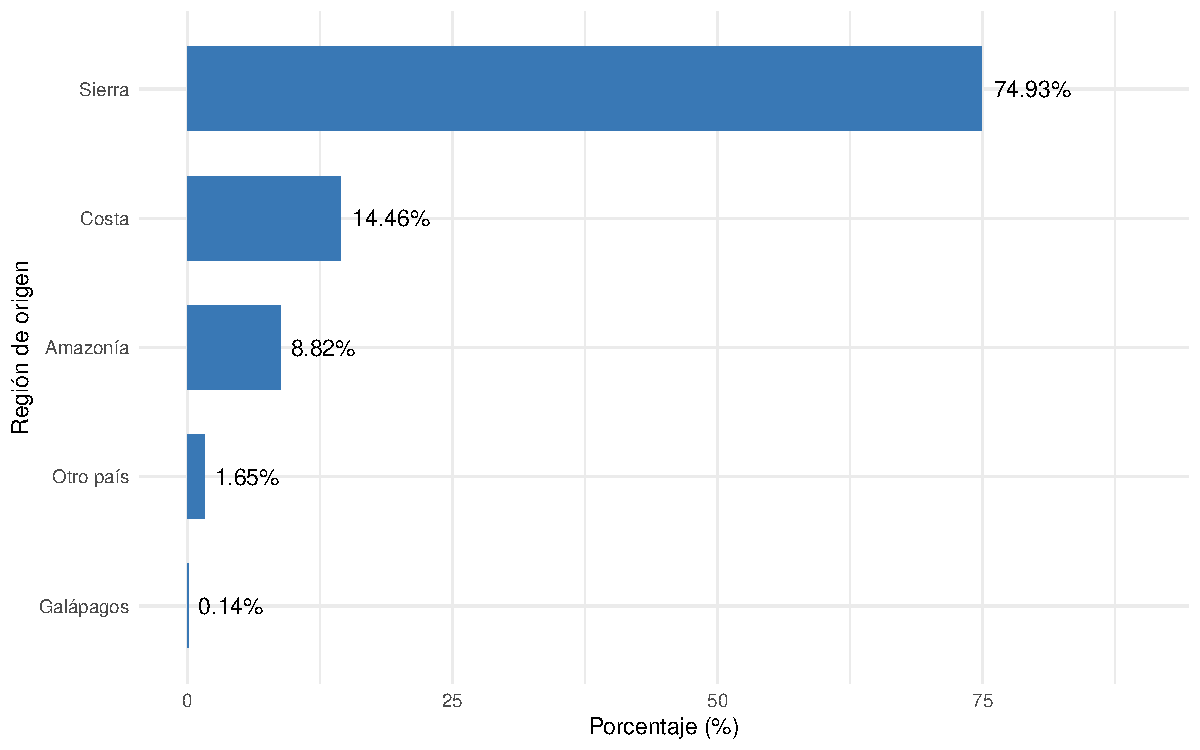
\includegraphics[keepaspectratio]{capitulos/Diagnóstico-territorial_files/figure-pdf/fig-region-origen-1.pdf}}

}

\caption{\label{fig-region-origen}Distribución porcentual de estudiantes
según región de origen}

\end{figure}%

Los resultados muestran que el 74,93 \% de los estudiantes encuestados
proviene de la región Sierra, seguida de la Costa con el 14,46 \% y la
Amazonía con el 8,82 \%. En menor proporción se encuentran los
estudiantes procedentes de otros países (1,65 \%) y Galápagos (0,14 \%).
Esta distribución evidencia una marcada concentración de estudiantes de
la Sierra, lo cual puede relacionarse con la ubicación geográfica de la
Universidad Nacional de Loja y su cercanía con las provincias de esta
región. Sin embargo, la presencia de estudiantes de otras regiones
refleja la diversidad territorial de la población universitaria, aspecto
importante para comprender los diferentes contextos sociales y
culturales en los que se desarrollan las percepciones sobre la violencia
basada en género.

\section{Distribución de los estudiantes según zona de
origen}\label{distribuciuxf3n-de-los-estudiantes-seguxfan-zona-de-origen}

La distribución de los estudiantes según su zona de origen permite
identificar la participación de la población procedente de áreas urbanas
y rurales. Esta diferenciación resulta importante para comprender la
diversidad territorial de la comunidad universitaria, considerando que
las condiciones sociales, económicas y culturales pueden variar entre
ambos espacios e influir en las percepciones sobre la violencia basada
en género.

\begin{figure}

\centering{

\pandocbounded{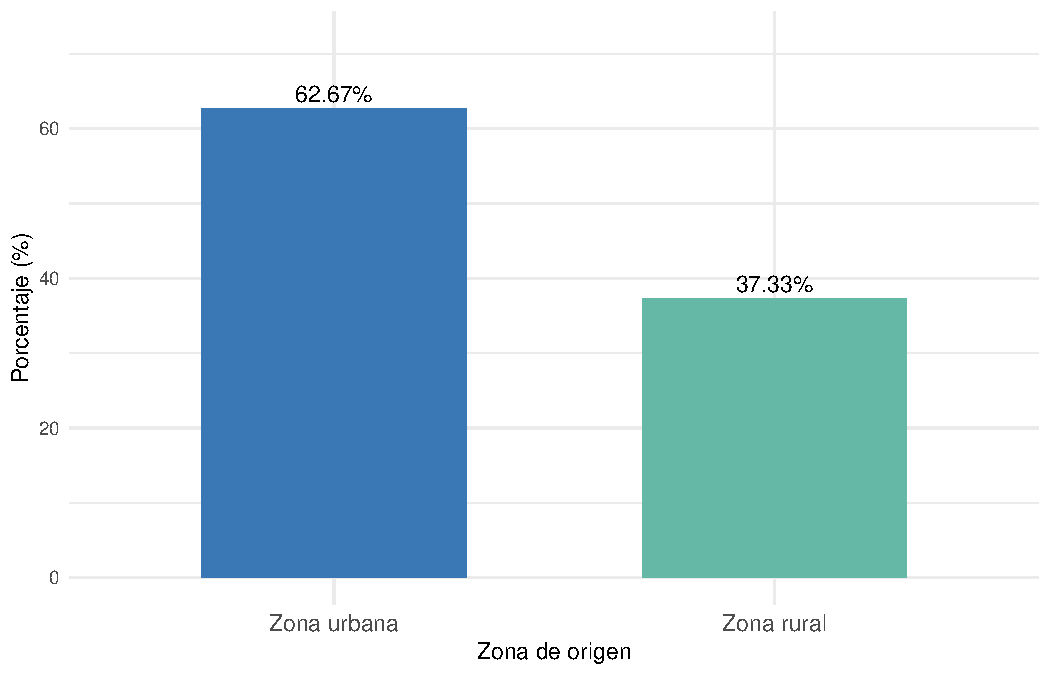
\includegraphics[keepaspectratio]{capitulos/Diagnóstico-territorial_files/figure-pdf/fig-zona-origen-1.pdf}}

}

\caption{\label{fig-zona-origen}Distribución porcentual de los
estudiantes según zona de origen}

\end{figure}%

Los resultados muestran que el 62,67 \% de los estudiantes encuestados
proviene de zonas urbanas, mientras que el 37,33 \% corresponde a zonas
rurales. Esta distribución evidencia una mayor participación de
estudiantes de procedencia urbana dentro de la muestra analizada. Sin
embargo, esta diferencia no permite afirmar por sí sola que los
estudiantes de zonas rurales tengan menores oportunidades de acceso a la
educación superior, puesto que sería necesario considerar otros
factores, como la distribución poblacional, las condiciones económicas y
las oportunidades educativas de cada territorio.

Desde la perspectiva de la violencia basada en género, la procedencia
territorial constituye una característica relevante para el análisis,
debido a que los estudiantes pueden desarrollarse en contextos sociales
y culturales diferentes. No obstante, los porcentajes presentados
únicamente describen la composición territorial de la muestra y no
permiten determinar si existen diferencias en las actitudes frente a la
violencia basada en género entre estudiantes urbanos y rurales. Para
establecer esta relación sería necesario comparar directamente las
respuestas de ambos grupos mediante un análisis estadístico.

\bookmarksetup{startatroot}

\chapter{Problemas y potencialidades}\label{problemas-y-potencialidades}

\section{Identificación de problemas y
potencialidades}\label{identificaciuxf3n-de-problemas-y-potencialidades}

A partir del diagnóstico sectorial y territorial realizado a los
estudiantes de la Universidad Nacional de Loja, se identifican
diferentes problemas y potencialidades relacionados con las actitudes
frente a la violencia basada en género. Este análisis permite reconocer
aspectos que requieren mayor atención, así como condiciones favorables
que pueden contribuir al desarrollo de estrategias de prevención,
sensibilización y fortalecimiento de la convivencia universitaria.

\section{Principales problemas
identificados}\label{principales-problemas-identificados}

\begin{itemize}
\tightlist
\item
  \textbf{\emph{Persistencia de actitudes que no expresan un rechazo
  pleno a la violencia basada en género}}
\end{itemize}

Aunque el 76,79 \% de los estudiantes seleccionó la categoría 5 ante la
afirmación «La violencia basada en género es inaceptable», el 23,21 \%
restante se distribuye entre las categorías inferiores. Esto evidencia
que no todos los estudiantes manifiestan el mismo nivel de aceptación de
dicha afirmación, por lo que resulta importante profundizar en sus
percepciones y fortalecer los procesos de sensibilización.

\begin{itemize}
\tightlist
\item
  \textbf{\emph{Diferencias en las condiciones socioeconómicas de los
  estudiantes}}
\end{itemize}

Los resultados muestran que el 48,83 \% de los encuestados combina sus
estudios con actividades laborales. Esta situación refleja la existencia
de responsabilidades económicas que pueden dificultar la participación
en actividades universitarias complementarias, incluidos los programas
de prevención y sensibilización sobre violencia basada en género.

\begin{itemize}
\tightlist
\item
  \textbf{\emph{Desigualdades territoriales en la procedencia
  estudiantil}}
\end{itemize}

El 62,67 \% de los estudiantes proviene de zonas urbanas, mientras que
el 37,33 \% procede de zonas rurales. Esta diferencia evidencia una
menor representación de estudiantes rurales en la población encuestada,
aunque por sí sola no permite determinar si existen barreras de acceso a
la educación superior o mayores niveles de violencia en estos
territorios.

\begin{itemize}
\tightlist
\item
  \textbf{\emph{Diversidad de contextos sociales y culturales}}
\end{itemize}

La procedencia de estudiantes de diferentes regiones del país implica la
convivencia de experiencias y entornos socioculturales diversos. Esto
plantea el desafío de desarrollar estrategias de prevención que
consideren las distintas realidades de la comunidad universitaria.

\section{Principales potencialidades
identificadas}\label{principales-potencialidades-identificadas}

\begin{itemize}
\tightlist
\item
  \textbf{\emph{Predominio de respuestas favorables al rechazo de la
  violencia basada en género}}
\end{itemize}

La concentración del 76,79 \% de respuestas en la categoría 5 constituye
una condición favorable para promover una cultura universitaria basada
en el respeto y la igualdad, siempre que esta categoría represente el
máximo grado de acuerdo con la afirmación evaluada.

\begin{itemize}
\tightlist
\item
  \emph{Participación de estudiantes de diferentes niveles académicos}
\end{itemize}

La presencia de estudiantes de nivel inicial, intermedio y final permite
desarrollar estrategias de sensibilización durante las distintas etapas
de la formación universitaria, favoreciendo la continuidad de las
acciones preventivas.

\begin{itemize}
\tightlist
\item
  \textbf{\emph{Diversidad territorial de la población universitaria}}
\end{itemize}

Aunque predomina la región Sierra con el 74,93 \%, también existe
participación de estudiantes de la Costa (14,46 \%), Amazonía (8,82 \%),
otros países (1,65 \%) y Galápagos (0,14 \%). Esta diversidad representa
una oportunidad para fomentar el intercambio de experiencias y promover
una comprensión más amplia de la violencia basada en género.

\begin{itemize}
\tightlist
\item
  \textbf{\emph{Disponibilidad de información para orientar
  intervenciones}}
\end{itemize}

La encuesta aplicada a 1.452 estudiantes proporciona información sobre
características demográficas, académicas, socioeconómicas y
territoriales, lo que constituye una base para identificar grupos de
interés y diseñar acciones de prevención más ajustadas a las
características de la población universitaria.

\bookmarksetup{startatroot}

\chapter{Evidencia emprírica}\label{evidencia-empruxedrica}

\section{Objetivo del análisis}\label{objetivo-del-anuxe1lisis}

El presente análisis empírico tiene como finalidad examinar la
asociación entre el nivel de avance académico y las actitudes frente a
la violencia basada en género en los estudiantes de la Universidad
Nacional de Loja. Para ello, se utiliza la información obtenida mediante
la encuesta estudiantil, considerando la percepción sobre si la
violencia basada en género es inaceptable y el nivel académico de los
encuestados. A través de herramientas estadísticas se busca identificar
si existen diferencias significativas entre los grupos estudiados,
complementando los resultados descriptivos presentados en los
diagnósticos sectorial y territorial.

\section{Muestra de análisis}\label{muestra-de-anuxe1lisis}

La base de datos utilizada contiene 1.452 registros de estudiantes de la
Universidad Nacional de Loja. Para el análisis empírico se consideran
las observaciones que presentan información válida tanto en la variable
de actitudes frente a la violencia basada en género como en el nivel de
avance académico. Esta selección permite realizar comparaciones entre
los estudiantes de nivel inicial, intermedio y final, evitando que los
valores faltantes afecten los cálculos estadísticos.

\textbf{\emph{Hipótesis nula (H₀):}} El nivel de avance académico y las
actitudes frente a la violencia basada en género son independientes.

\textbf{\emph{Hipótesis alternativa (H₁):}} Existe una asociación entre
el nivel de avance académico y las actitudes frente a la violencia
basada en género.

\section{Asociación general}\label{asociaciuxf3n-general}

Para examinar la relación entre el nivel de avance académico y las
actitudes frente a la violencia basada en género, se aplicó la prueba
chi-cuadrado de independencia, utilizando 1.442 observaciones válidas de
estudiantes de la Universidad Nacional de Loja. Los resultados muestran
un estadístico chi-cuadrado de 12,376, con 8 grados de libertad y un
valor p de 0,1352. Dado que este valor es superior al nivel de
significancia del 5 \%, no se rechaza la hipótesis nula de independencia
entre las variables. Por lo tanto, no se encuentra evidencia
estadísticamente significativa de una asociación entre el nivel
académico y las respuestas sobre la inaceptabilidad de la violencia
basada en género. Esto sugiere que las diferencias observadas entre
estudiantes de nivel inicial, intermedio y final podrían responder a
variaciones muestrales y no necesariamente a una relación sistemática
entre ambas variables.

\section{Intensidad de la
asociación}\label{intensidad-de-la-asociaciuxf3n}

El coeficiente V de Cramér presenta un valor aproximado de 0,0655, lo
que indica una asociación de magnitud muy débil entre el nivel académico
y las actitudes frente a la violencia basada en género. Este resultado
complementa la prueba chi-cuadrado y muestra que las diferencias entre
los niveles académicos son reducidas. En consecuencia, el avance en la
formación universitaria no presenta una asociación estadísticamente
significativa con las respuestas analizadas, aunque esto no permite
descartar la influencia de otros factores personales, sociales o
educativos.

\section{Asociación según sexo}\label{asociaciuxf3n-seguxfan-sexo}

Para complementar el análisis empírico, se examinó la asociación entre
el sexo de los estudiantes y las actitudes frente a la violencia basada
en género. Se utilizaron 1.452 observaciones válidas y se aplicó
inicialmente la prueba chi-cuadrado de independencia, obteniendo un
estadístico de 8,5147 con 8 grados de libertad. Debido a la presencia de
frecuencias esperadas reducidas en algunas categorías, se consideró
necesario utilizar una simulación de Monte Carlo para evaluar la
significancia estadística de la asociación. Este procedimiento permite
analizar las posibles diferencias entre las respuestas de los
estudiantes sin atribuirlas directamente a su sexo.

\section{Asociación según zona de
origen}\label{asociaciuxf3n-seguxfan-zona-de-origen}

Con el propósito de incorporar la dimensión territorial en el análisis
empírico, se examinó la asociación entre la zona de origen de los
estudiantes y sus actitudes frente a la violencia basada en género,
considerando 1.452 observaciones válidas. Para ello, se aplicó la prueba
chi-cuadrado de independencia, obteniendo un estadístico de 5,8352 con 4
grados de libertad y un valor p de 0,2118. Debido a que este valor
supera el nivel de significancia del 5 \%, no se rechaza la hipótesis
nula de independencia entre las variables. Por lo tanto, no se encontró
evidencia estadísticamente significativa de diferencias en la
distribución de las respuestas entre estudiantes provenientes de zonas
urbanas y rurales. Esto sugiere que, dentro de la muestra analizada, la
zona de origen no presenta una asociación estadísticamente significativa
con las actitudes frente a la violencia basada en género, aunque no se
descarta la posible influencia de otros factores sociales, culturales o
educativos.

\section{Limitaciones}\label{limitaciones}

Los resultados obtenidos deben interpretarse considerando algunas
limitaciones metodológicas. En primer lugar, la información corresponde
a una encuesta aplicada a estudiantes de la Universidad Nacional de
Loja, por lo que las asociaciones identificadas no permiten establecer
relaciones de causalidad. Asimismo, las actitudes frente a la violencia
basada en género se analizan a partir de respuestas declaradas por los
encuestados, las cuales pueden estar influenciadas por factores
personales y sociales. Por otra parte, la distribución desigual de
observaciones entre determinadas categorías puede afectar la precisión
de las pruebas estadísticas. Finalmente, los resultados reflejan las
características de la población estudiantil encuestada y no
necesariamente representan las percepciones de estudiantes de otras
instituciones de educación superior.

\section{Interpretación general}\label{interpretaciuxf3n-general}

El análisis empírico tiene como finalidad determinar si existe una
asociación estadísticamente significativa entre el nivel de avance
académico y las actitudes frente a la violencia basada en género en los
estudiantes de la Universidad Nacional de Loja. Para ello, se consideran
las respuestas de 1.442 estudiantes con información disponible en ambas
variables y se emplea la prueba de independencia chi-cuadrado,
complementada con el coeficiente V de Cramér para evaluar la intensidad
de la asociación.

Los resultados muestran un valor p de 0,1352, superior al nivel de
significancia establecido de 0,05. Por tanto, no se rechaza la hipótesis
nula de independencia entre las variables, lo que indica que no se
encontró evidencia estadística suficiente para afirmar que las actitudes
frente a la violencia basada en género difieren según el nivel de avance
académico.

Asimismo, el coeficiente V de Cramér presenta un valor de 0,0655, lo que
evidencia una asociación de magnitud muy débil entre las variables
analizadas. Este resultado complementa la prueba de chi-cuadrado y
sugiere que las diferencias observadas entre los niveles académicos son
reducidas.

En consecuencia, los resultados no respaldan la existencia de una
asociación estadísticamente significativa entre el avance académico y
las actitudes frente a la violencia basada en género en la muestra
estudiada. Sin embargo, esto no significa que ambas variables sean
necesariamente independientes en toda la población universitaria, sino
que, con la información y los procedimientos utilizados, no se obtuvo
evidencia suficiente para establecer dicha asociación.

\bookmarksetup{startatroot}

\chapter{Revisión de la Literatura}\label{revisiuxf3n-de-la-literatura}

La relación entre la formación académica y las actitudes frente a la
violencia basada en género requiere considerar que el acceso a la
educación superior no implica necesariamente una transformación de las
creencias adquiridas en otros espacios sociales. Balatacı et~al. (2026)
examinan las actitudes hacia la violencia en las relaciones de pareja y
su relación con los roles de género entre universitarios, mientras que
Patwary \& Esha (2025) estudian la interacción entre educación y normas
comunitarias en la justificación de la violencia de pareja. En una
perspectiva similar, Banda et~al. (2025) abordan la desigualdad
educativa y las normas de género como elementos relacionados con esta
problemática. Estos enfoques permiten reconocer que la educación formal
constituye una dimensión relevante, pero no puede analizarse de manera
aislada de las normas sociales que influyen en las percepciones
individuales. Por ello, la permanencia en la universidad no
necesariamente supone un rechazo progresivo y uniforme de todas las
manifestaciones de violencia.

Las diferencias entre actitudes también pueden explicarse por la manera
en que las personas interpretan los roles de género y las relaciones
interpersonales. Yildirim-Hamurcu \& Terzioglu (2023) estudian las
actitudes hacia la violencia en el noviazgo entre universitarios turcos,
mientras que Alp Yilmaz \& Şener Taplak (2021) relacionan estas
actitudes con la autoestima y la percepción de género. Por su parte,
Şahin Altun et~al. (2025) examinan el papel mediador de la autoeficacia
en la relación entre las actitudes hacia la violencia contra las mujeres
y la flexibilidad cognitiva. Estas investigaciones incorporan
dimensiones que no se encuentran representadas directamente por el nivel
académico, lo que permite comprender por qué estudiantes que cursan
semestres similares pueden mantener percepciones diferentes. En
consecuencia, el avance académico debe entenderse como una
característica de la trayectoria educativa y no como una medida directa
de la transformación de las creencias sobre violencia de género.

Un aspecto particularmente importante es que el rechazo general hacia la
violencia no necesariamente implica el reconocimiento de todas las
conductas que pueden constituirla. Bonilla-Algovia et~al. (2024)
desarrollan una escala para evaluar creencias estereotipadas sobre la
violencia basada en género, mientras que Güner et~al. (2026) analizan la
relación entre percepción de género y aceptación de mitos sobre la
violencia en el noviazgo entre estudiantes de ciencias de la salud.
Sezer et~al. (2026) también estudian la autoestima y las creencias
relacionadas con estos mitos, y Atasever \& Taşçı Duran (2026) proponen
una aproximación gamificada para medir actitudes hacia la violencia en
las relaciones de pareja. Estos trabajos permiten identificar una
limitación importante de las preguntas generales: una persona puede
considerar inaceptable la violencia y, al mismo tiempo, mantener
percepciones que minimicen determinadas agresiones. Por ello, la
interpretación de las respuestas debe considerar qué aspecto específico
de la violencia mide cada instrumento.

Esta distinción también aparece en investigaciones centradas en la
dependencia emocional y las formas menos visibles de violencia.
Castillo-Gonzáles et~al. (2024) examinan la relación entre violencia en
el noviazgo y dependencia emocional, mientras que Şener \& Günaydın
(2026) incorporan factores como el impacto social y la dificultad para
identificar y expresar emociones. Weathers \& Gangel (2025), por su
parte, estudian las percepciones universitarias sobre el abuso digital
en las relaciones de pareja desde la teoría de los esquemas de género.
Coppola et~al. (2025) analizan las representaciones psicosociales de la
violencia basada en género entre estudiantes universitarios italianos.
En conjunto, estos antecedentes permiten considerar que las actitudes no
constituyen una dimensión completamente uniforme, puesto que pueden
variar según el tipo de comportamiento, la relación interpersonal y las
creencias utilizadas para interpretarlo.

Las experiencias previas también representan una dimensión que debe
distinguirse de la formación universitaria. You \& Kwon (2023)
investigan la influencia de la exposición directa e indirecta a la
violencia doméstica sobre la victimización en las relaciones de pareja,
mientras que Rueda et~al. (2026) examinan experiencias de victimización,
estrés y comportamientos asociados con la ruptura de relaciones entre
universitarios. Rechenberg et~al. (2024) estudian el estigma relacionado
con el género hacia personas que experimentaron violencia sexual o
física durante la infancia. Estos trabajos permiten situar las
percepciones y experiencias de los estudiantes dentro de trayectorias
personales más amplias. No obstante, es importante diferenciar los
antecedentes de victimización de las actitudes declaradas, debido a que
ambas dimensiones requieren indicadores específicos y no pueden
considerarse equivalentes.

La literatura también muestra la importancia de estudiar las condiciones
en las que se presenta la violencia dentro de las instituciones de
educación superior. Wellum et~al. (2023) investigan la prevalencia y los
factores de riesgo de agresión sexual entre universitarios de los Países
Bajos, mientras que Li et~al. (2023) examinan experiencias de acoso
sexual y estrategias de respuesta entre estudiantes chinos. Adhia et~al.
(2023) analizan la violencia sexual y su denuncia formal entre
estudiantes deportistas, y Kaufmann et~al. (2026) abordan la
discriminación, el acoso persistente, el acoso sexual y la violencia
sexual en el entorno universitario. Aunque estas investigaciones se
concentran principalmente en experiencias de violencia, permiten
comprender que las universidades constituyen espacios donde las
relaciones de género deben examinarse tanto desde las percepciones
estudiantiles como desde las condiciones institucionales que pueden
favorecer o dificultar su reconocimiento.

En este contexto, una actitud contraria a la violencia no garantiza
necesariamente la disposición a denunciarla. Lathan et~al. (2023)
estudian la aceptación de mitos sobre la violación y otras barreras para
presentar denuncias formales, mientras que Pinchevsky \& Hayes (2023)
analizan el conocimiento estudiantil sobre las políticas y
procedimientos relacionados con conductas sexuales inapropiadas. Nystrom
\& Richards (2023) examinan las políticas universitarias sobre
relaciones sexuales consensuadas entre docentes y estudiantes, y Ellyson
et~al. (2023) estudian las políticas de amnistía por consumo de
sustancias y su relación con la denuncia de violencia sexual. Estas
investigaciones permiten diferenciar el reconocimiento de una conducta
violenta, el conocimiento de los mecanismos institucionales y la
decisión de utilizarlos. La distinción es relevante porque las
respuestas de rechazo en una encuesta no permiten establecer, por sí
solas, cómo actuarían los estudiantes ante una situación real.

La búsqueda de ayuda constituye otra dimensión relacionada con las
respuestas frente a la violencia. Wood et~al. (2025) examinan las
actitudes hacia la búsqueda de apoyo ante la violencia de pareja en la
República Democrática del Congo, mientras que Jung \& Dlamini (2024)
investigan las intenciones de solicitar ayuda profesional entre
estudiantes universitarias de Eswatini. Owusu-Antwi et~al. (2024)
abordan la violencia basada en género y los factores relacionados con la
búsqueda de ayuda entre universitarios del África subsahariana. Por su
parte, Zhang et~al. (2024) estudian la relación entre malestar
psicológico, experiencias abusivas y búsqueda de apoyo. Estos
antecedentes permiten comprender que el rechazo hacia la violencia y la
utilización de servicios de atención corresponden a decisiones
diferentes. En consecuencia, las estrategias institucionales deben
considerar no solamente la sensibilización, sino también las condiciones
que facilitan el acceso a orientación y acompañamiento.

La respuesta colectiva también tiene importancia dentro del entorno
universitario. Hoxmeier et~al. (2023) analizan la participación de
estudiantes en conversaciones sobre prevención de la violencia con sus
compañeros, mientras que Fedina et~al. (2023) estudian la formación y
preparación para responder ante situaciones de violencia de pareja entre
estudiantes, docentes y personal universitario. Svalin et~al. (2026)
examinan las actitudes y la disposición a intervenir frente a la
violencia contra las mujeres, y Clerincx et~al. (2025) investigan las
barreras para adoptar comportamientos positivos como observadores ante
situaciones de violencia basada en género. Estos enfoques permiten
distinguir entre expresar una postura de rechazo y asumir una
responsabilidad activa frente a conductas violentas. Por ello, la
prevención universitaria no debería limitarse a promover respuestas
favorables en encuestas, sino también fortalecer las capacidades de
identificación, intervención y apoyo.

Las investigaciones sobre programas preventivos aportan elementos
adicionales para interpretar el papel de la educación. Reyal et~al.
(2024) examinan una intervención comunitaria participativa relacionada
con conocimientos, actitudes y prácticas frente a la violencia de
pareja. Butler et~al. (2024) estudian el programa Mentors in Violence
Prevention y su relación con los conocimientos y actitudes
estudiantiles. Bloom et~al. (2023) analizan una intervención dirigida a
personas cercanas a sobrevivientes de violencia de pareja en campus
universitarios, mientras que Barata et~al. (2025) examinan un programa
de resistencia a la agresión sexual y sus efectos sobre la violencia de
pareja. Asimismo, DaSilva-Ibru et~al. (2025) estudian intervenciones
dirigidas a adolescentes y hombres jóvenes en países de ingresos bajos y
medios, y Łyś et~al. (2026) abordan un programa digital de prevención
considerando el esencialismo de género, el sexismo ambivalente y la
percepción de respuesta universitaria. Estos antecedentes permiten
reconocer una diferencia fundamental: el avance regular en una carrera
no equivale necesariamente a recibir formación específica sobre
prevención de la violencia basada en género.

La diversidad de la población estudiantil también debe considerarse al
interpretar las actitudes. O'Connor et~al. (2023) estudian patrones de
victimización y revelación de experiencias de violencia entre
universitarios latinos transgénero y cisgénero, mientras que Wilson-Yang
et~al. (2026) examinan la prevalencia y las consecuencias de la
violencia basada en género entre estudiantes trans y de género diverso
en Ontario. En Ecuador, Vara-Horna et~al. (2025) investigan la violencia
contra estudiantes LGBTQ+ y sus consecuencias emocionales y educativas.
Estos antecedentes permiten reconocer que las experiencias de violencia
pueden diferir entre grupos y que las características individuales deben
considerarse al analizar la realidad universitaria. Sin embargo, las
diferencias en experiencias de victimización no permiten deducir
automáticamente diferencias en las actitudes de rechazo, por lo que
ambas dimensiones deben mantenerse separadas durante la interpretación.

En relación con las consecuencias de la violencia, Fielding-Miller
et~al. (2024) examinan la asociación entre violencia sexual y depresión,
considerando el papel del apoyo social percibido entre universitarias de
Eswatini. Laz-Figueroa et~al. (2025) estudian la relación entre
violencia basada en género y salud mental de estudiantes universitarias.
Por su parte, Mokaya et~al. (2025) desarrollan un estudio fenomenológico
sobre violencia basada en género en el entorno educativo. Estas
investigaciones permiten comprender que la problemática no se limita a
las agresiones visibles, sino que también puede involucrar consecuencias
psicológicas y dificultades en la experiencia educativa. No obstante,
para la presente investigación resulta indispensable distinguir entre
las consecuencias de haber experimentado violencia y las actitudes hacia
su aceptación o rechazo, puesto que el análisis estadístico realizado en
la Universidad Nacional de Loja se concentra en esta última dimensión.

Las condiciones sociales y económicas representan otro aspecto que puede
intervenir en la construcción de las percepciones. Adu et~al. (2022)
examinan factores sociodemográficos y económicos relacionados con la
justificación de la violencia de pareja, mientras que Demissie et~al.
(2025) estudian la justificación de la violencia física de pareja entre
hombres casados de África oriental. Kelecha et~al. (2024) analizan
normas de género inequitativas y sus factores asociados entre
universitarios del sur de Etiopía. Estos antecedentes permiten reconocer
que las creencias sobre la violencia pueden relacionarse con contextos
sociales que trascienden la formación académica. Sin embargo, sus
resultados no deben trasladarse directamente a los estudiantes
ecuatorianos, debido a las diferencias entre poblaciones, instrumentos y
contextos de estudio. Su utilidad consiste en fundamentar la inclusión
de características sociodemográficas como dimensiones de análisis, sin
asumir relaciones que no hayan sido comprobadas en la muestra
investigada.

La procedencia territorial y la diversidad cultural también pueden
influir en las experiencias de socialización de los estudiantes. Kennedy
et~al. (2024) examinan las perspectivas de universitarios culturalmente
diversos sobre las políticas de violencia sexual y la necesidad de
enfoques preventivos sensibles a esas diferencias. En una línea
complementaria, Muñoz-Aucapiña et~al. (2025) abordan la validación
psicométrica de un cuestionario sobre violencia en el noviazgo en
población ecuatoriana, lo que resalta la importancia de utilizar
instrumentos adecuados al contexto de aplicación. Estos trabajos
permiten comprender que las diferencias culturales deben considerarse
tanto en el diseño de estrategias preventivas como en la interpretación
de las respuestas. No obstante, la procedencia urbana o rural no debe
entenderse como un indicador automático de mayor o menor tolerancia
hacia la violencia, sino como una característica cuya asociación
requiere evidencia empírica.

En conjunto, las investigaciones revisadas muestran que la violencia
basada en género ha sido estudiada desde sus manifestaciones, los
factores que contribuyen a justificarla, las experiencias de
victimización, las consecuencias psicológicas y las estrategias de
prevención. Sin embargo, estos enfoques no son equivalentes a evaluar si
las actitudes de rechazo cambian según el avance académico. Esta
diferencia constituye un aspecto central para el presente trabajo,
debido a que el semestre cursado representa una característica de la
trayectoria universitaria, pero no mide directamente los conocimientos
sobre igualdad de género, la participación en programas preventivos ni
las experiencias personales de los estudiantes.

En este sentido, la investigación realizada en la Universidad Nacional
de Loja aporta evidencia específica mediante el análisis de las
actitudes frente a la violencia basada en género y su relación con los
niveles inicial, intermedio y final de formación. Los resultados
descriptivos muestran que el 76,79 \% de los encuestados seleccionó la
categoría de mayor rechazo hacia la violencia, lo que evidencia una
concentración importante de respuestas favorables a su desaprobación.
Sin embargo, la prueba de chi-cuadrado presentó un valor p de 0,1352 y
el coeficiente V de Cramér fue de 0,0655, por lo que no se identificó
una asociación estadísticamente significativa entre el avance académico
y las actitudes analizadas, y la magnitud de la relación observada fue
muy débil. Estos resultados no demuestran que la educación universitaria
carezca de importancia, sino que el nivel de avance académico,
considerado de manera aislada, no permitió identificar diferencias
estadísticamente significativas en las respuestas de la muestra.

Por tanto, la principal contribución de la literatura al presente
estudio consiste en mostrar que las actitudes frente a la violencia
basada en género responden a una combinación de dimensiones educativas,
sociales, culturales e individuales. Los antecedentes permiten
interpretar con mayor precisión la ausencia de asociación estadística
encontrada, sin atribuirla automáticamente a la falta de formación o de
sensibilización. Asimismo, refuerzan la necesidad de desarrollar
estrategias preventivas dirigidas a estudiantes de todos los niveles
académicos, considerando que la permanencia en la universidad no
garantiza por sí misma una transformación de las creencias. De esta
manera, la investigación contribuye a comprender las actitudes de
rechazo hacia la violencia basada en género dentro de la comunidad
estudiantil de la Universidad Nacional de Loja y establece una base para
futuros análisis que incorporen otras variables relacionadas con las
normas sociales, las experiencias personales y la formación específica
en igualdad de género.

\bookmarksetup{startatroot}

\chapter*{Referencias}\label{referencias}
\addcontentsline{toc}{chapter}{Referencias}

\markboth{Referencias}{Referencias}

\protect\phantomsection\label{refs}
\begin{CSLReferences}{1}{0}
\bibitem[\citeproctext]{ref-art13}
Adhia, A., Ellyson, A. M., \& Kroshus, E. (2023). Prevalence and Formal
Reporting of Sexual Violence among Undergraduate Student-Athletes.
\emph{Journal of Interpersonal Violence}.
\url{https://doi.org/10.1177/08862605221081936}

\bibitem[\citeproctext]{ref-art23}
Adu, C., Asare, B. Y.-A., Agyemang-Duah, W., Adomako, E. B., Agyekum, A.
K., \& Peprah, P. (2022). Impact of socio-demographic and economic
factors on intimate partner violence justification among women in union
in Papua New Guinea. \emph{Pendiente de confirmar}.
\url{https://doi.org/10.1186/s13690-022-00889-0}

\bibitem[\citeproctext]{ref-art40}
Alp Yilmaz, F., \& Şener Taplak, A. (2021). Relationship between
self-esteem perception of gender and attitudes towards dating violence
among university students. \emph{Perspectives in Psychiatric Care}.
\url{https://doi.org/10.1111/ppc.12634}

\bibitem[\citeproctext]{ref-art26}
Atasever, I., \& Taşçı Duran, E. (2026). A Novel Gamified Approach to
Measuring Dating Violence Attitudes. \emph{Violence Against Women}.
\url{https://doi.org/10.1177/10778012261495052}

\bibitem[\citeproctext]{ref-art01}
Balatacı, U., Ay, B., Tarhan, R., \& Ay, A. (2026). Attitudes toward
dating violence and their relationship with gender role attitudes among
university students. \emph{BMC Public Health}.
\url{https://doi.org/10.1186/s12889-026-28542-3}

\bibitem[\citeproctext]{ref-art32}
Banda, L. O. L., Mwaene, E., Banda, C. V., \& Banda, J. T. (2025).
Breaking the cycle how educational inequality and gender norms fuel
intimate-partner violence in Kiribati. \emph{BMC Public Health}.
\url{https://doi.org/10.1186/s12889-025-25190-x}

\bibitem[\citeproctext]{ref-art47}
Barata, P. C., Samardzic, T., Eliasziw, M., Senn, C. Y., Radtke, H. L.,
Hobden, K. L., \& Thurston, W. E. (2025). A Successful Sexual Assault
Resistance Program Also Reduced Intimate Partner Violence. \emph{Journal
of Interpersonal Violence}.
\url{https://doi.org/10.1177/08862605241270057}

\bibitem[\citeproctext]{ref-art29}
Bloom, T. L., Perrin, N., Brown, M. L., Campbell, J., Clough, A., Grace,
K. T., Laughon, K., Messing, J., Eden, K. B., Turner, R., \& Glass, N.
(2023). Concerned friends of intimate partner violence survivors results
from the myPlan randomized controlled trial on college campuses.
\emph{BMC Public Health}.
\url{https://doi.org/10.1186/s12889-023-15918-y}

\bibitem[\citeproctext]{ref-art22}
Bonilla-Algovia, E., Pana, A. G., \& Carrasco Carpio, C. (2024). Design
and Validation of the Gender-Based Violence Stereotypical Beliefs Scale.
\emph{Behavioral Sciences}. \url{https://doi.org/10.3390/bs14111093}

\bibitem[\citeproctext]{ref-art28}
Butler, N., Quigg, Z., Wilson, C., McCoy, E., \& Bates, R. (2024). The
Mentors in Violence Prevention programme impact on students knowledge
and attitudes. \emph{BMC Public Health}.
\url{https://doi.org/10.1186/s12889-024-18210-9}

\bibitem[\citeproctext]{ref-art37}
Castillo-Gonzáles, M., Mendo-Lázaro, S., León-del-Barco, B.,
Terán-Andrade, E., \& López-Ramos, V.-M. (2024). Dating Violence and
Emotional Dependence in University Students. \emph{Behavioral Sciences}.
\url{https://doi.org/10.3390/bs14030176}

\bibitem[\citeproctext]{ref-Clerincx_2025}
Clerincx, T., Schaillée, H., \& Derom, I. (2025). Barriers to positive
bystander behavior: understanding undergraduate physical education
students' attitudes and intentional behavior in gender-based violence
prevention. \emph{Frontiers in Sports and Active Living}, \emph{7}.
\url{https://doi.org/10.3389/fspor.2025.1569307}

\bibitem[\citeproctext]{ref-art43}
Coppola, I., Tironi, M., Berlin, E., Scudieri, L., Bizzi, F., Rollero,
C., \& Rania, N. (2025). Psychosocial Representations of Gender-Based
Violence Among University Students from Northwestern Italy.
\emph{Behavioral Sciences}. \url{https://doi.org/10.3390/bs15101373}

\bibitem[\citeproctext]{ref-art34}
DaSilva-Ibru, A. K., Stöckl, H., Pearson, I., \& Zimmerman, C. (2025).
Interventions for adolescent school boys and young men to reduce
gender-based violence in low- and middle-income countries. \emph{BMC
Public Health}. \url{https://doi.org/10.1186/s12889-025-25184-9}

\bibitem[\citeproctext]{ref-art20}
Demissie, K. A., Geberu, D. M., Teshale, G., Jejaw, M., Tiruneh, M. G.,
Tafere, T. Z., Hagos, A., \& Baffa, L. D. (2025). Justification of
physical intimate partner violence among married men in East Africa.
\emph{Frontiers in Sociology}.
\url{https://doi.org/10.3389/fsoc.2025.1514917}

\bibitem[\citeproctext]{ref-art15}
Ellyson, A. M., Ortega, A., \& Bedard-Gilligan, M. A. (2023).
Institution of Higher Education Substance Use Amnesty Policies and
Sexual Violence Reporting. \emph{Journal of Interpersonal Violence}.
\url{https://doi.org/10.1177/08862605221080156}

\bibitem[\citeproctext]{ref-art11}
Fedina, L., Barr, E., Ting, L., Shah, R., Chayhitz, M., Goodmark, L.,
Barth, R. P., \& Njie-Carr, V. P. S. (2023). Intimate Partner Violence
Training and Readiness to Respond among Students Staff and Faculty in
Three Institutions in the United States. \emph{Journal of Interpersonal
Violence}. \url{https://doi.org/10.1177/08862605221099948}

\bibitem[\citeproctext]{ref-art48}
Fielding-Miller, R., McDougal, L., Frost, E., Masuku, S., \& Shabalala,
F. (2024). Association between sexual violence and depression is
mediated by perceived social support among female university students in
the kingdom of Eswatini. \emph{BMC Public Health}.
\url{https://doi.org/10.1186/s12889-024-20040-8}

\bibitem[\citeproctext]{ref-G_ner_2026}
Güner, Ö., Karataş, B., Tunç, İ., \& Tufan, S. (2026). Does gender
perception influence the acceptance of dating violence myths among
health sciences students? \emph{BMC Public Health}, \emph{26}(1).
\url{https://doi.org/10.1186/s12889-026-27044-6}

\bibitem[\citeproctext]{ref-art06}
Hoxmeier, J. C., Connor, R. A., \& McMahon, S. (2023). College Students
Engagement in Violence Prevention Discussions with Peers. \emph{Journal
of Interpersonal Violence}.
\url{https://doi.org/10.1177/08862605221120901}

\bibitem[\citeproctext]{ref-Jung_2024}
Jung, M. S., \& Dlamini, N. S. (2024). Factors Influencing Professional
Help‐Seeking Intentions for Sexual and Gender‐Based Violence Among
Female University Students in Eswatini. \emph{Public Health Nursing},
\emph{42}(1), 325-333. \url{https://doi.org/10.1111/phn.13477}

\bibitem[\citeproctext]{ref-art31}
Kaufmann, M.-T., Preisendanz, N., Fegert, J. M., \& Clemens, V. (2026).
Discrimination stalking sexual harassment and sexual violence at the
university. \emph{BMC Public Health}.
\url{https://doi.org/10.1186/s12889-025-25864-6}

\bibitem[\citeproctext]{ref-Kelecha_2024}
Kelecha, Y. T., Ayele, A. A., Goda, H. S., Demissie, M. H., \& Toma, T.
M. (2024). Inequitable gender norms and its associated factors among
university students in southern Ethiopia: a cross-sectional study, 2022.
\emph{Frontiers in Public Health}, \emph{12}.
\url{https://doi.org/10.3389/fpubh.2024.1462782}

\bibitem[\citeproctext]{ref-art49}
Kennedy, K. D., Malinen, K., MacLeod, E., VanTassel, B., O'Rourke, K.,
\& Small Legs-Nagge, C. (2024). Culturally Diverse Students'
Perspectives on Sexual Violence Policies: Recommendations for Culturally
Sensitive Approaches to Prevention in Higher Education. \emph{Journal of
Interpersonal Violence}. \url{https://doi.org/10.1177/08862605241245372}

\bibitem[\citeproctext]{ref-art09}
Lathan, E. C., Koon-Magnin, S., Selwyn, C. N., Isaak, H., \&
Langhinrichsen-Rohling, J. (2023). Rape Myth Acceptance and Other
Barriers to Formally Reporting Sexual Assault Among College Students.
\emph{Journal of Interpersonal Violence}.
\url{https://doi.org/10.1177/08862605221137703}

\bibitem[\citeproctext]{ref-art38}
Laz-Figueroa, K., Sánchez, B. R. H., García, J. C. S., Guevara-Viejó,
F., \& Molina-Molina, V. (2025). Gender-based violence and its
relationship to the mental health of female university students.
\emph{Frontiers in Sociology}.
\url{https://doi.org/10.3389/fsoc.2025.1597261}

\bibitem[\citeproctext]{ref-art10}
Li, X., Gu, X., Ariyo, T., \& Jiang, Q. (2023). Understanding Experience
and Response Strategies to Sexual Harassment Among Chinese College
Students. \emph{Journal of Interpersonal Violence}.
\url{https://doi.org/10.1177/08862605221101183}

\bibitem[\citeproctext]{ref-art50}
Łyś, A. E., Bargiel-Matusiewicz, K., Zeuthen, K., Barbara, G., Cattaneo,
C., Collini, F., Horten, B., Pavlík, P., Pellizzone, I., Smetáčková, I.,
Ringhof, E. V., Visnu, A., \& Orth, M. (2026). The Potential
Effectiveness of an Online Gender-Based Violence Prevention Program for
European Students---The Role of Gender Essentialism, Ambivalent Sexism,
and Perceived Responsiveness of the University. \emph{Violence Against
Women}. \url{https://doi.org/10.1177/10778012251362224}

\bibitem[\citeproctext]{ref-art33}
Mokaya, A. G., Kikuvi, G., Mutai, J., \& Memiah, P. (2025). A
descriptive phenomenological study of school-related gender-based
violence. \emph{BMC Public Health}.
\url{https://doi.org/10.1186/s12889-025-25341-0}

\bibitem[\citeproctext]{ref-art45}
Muñoz-Aucapiña, M., Muñoz-Aucapiña, R., García-García, I.,
Álvarez-Serrano, M., Antolí-Jover, A., \& Martínez-García, E. (2025).
Psychometric Validation of the Dating Violence Questionnaire (DVQ-R) in
Ecuadorians. \emph{Behavioral Sciences}.
\url{https://doi.org/10.3390/bs15010068}

\bibitem[\citeproctext]{ref-art14}
Nystrom, A., \& Richards, T. N. (2023). Faculty-Student Consensual
Sexual Relationship Policies. \emph{Journal of Interpersonal Violence}.
\url{https://doi.org/10.1177/08862605221128054}

\bibitem[\citeproctext]{ref-art12}
O'Connor, J., Ganson, K. T., Ladonice, S., \& Cardenas, I. (2023).
Patterns of Violence Victimization and Disclosure Among Transgender and
Cisgender Latinx College Students. \emph{Journal of Interpersonal
Violence}. \url{https://doi.org/10.1177/08862605221127217}

\bibitem[\citeproctext]{ref-art36}
Owusu-Antwi, R., Fedina, L., Robba, M. J. B., Khatibi, K., Bosomtwe, D.,
Nsereko, E., Shadare, O., Compton, S., Akinyemi, A., Randa, M. B.,
Afolabi, A. A., \& Munro-Kramer, M. L. (2024). Prevalence of
gender-based violence and factors associated with help-seeking among
university students in sub-Saharan Africa. \emph{Women's Health}.
\url{https://doi.org/10.1177/17455057241307519}

\bibitem[\citeproctext]{ref-art02}
Patwary, M. H., \& Esha, S. N. (2025). Interplay of education and
community norms in justifying intimate partner violence among
ever-married women in Bangladesh. \emph{BMC Public Health}.
\url{https://doi.org/10.1186/s12889-025-22348-5}

\bibitem[\citeproctext]{ref-art07}
Pinchevsky, G. M., \& Hayes, B. E. (2023). Understanding College
Students Perceived Help-Seeking Knowledge and Awareness about Sexual
Misconduct Policies and Procedures. \emph{Journal of Interpersonal
Violence}. \url{https://doi.org/10.1177/08862605221081935}

\bibitem[\citeproctext]{ref-art30}
Rechenberg, T., Fleischer, T., Sander, C., \& Schomerus, G. (2024).
Gender-related stigma toward individuals with a history of sexual or
physical violence in childhood. \emph{BMC Public Health}.
\url{https://doi.org/10.1186/s12889-024-19913-9}

\bibitem[\citeproctext]{ref-art03}
Reyal, H. P., Perera, M. N., \& Guruge, G. N. D. (2024). Effectiveness
of a community-based participatory health promotion intervention to
address knowledge attitudes and practices related to intimate partner
violence. \emph{BMC Public Health}.
\url{https://doi.org/10.1186/s12889-024-18893-0}

\bibitem[\citeproctext]{ref-art17}
Rueda, G., Ayora, D., Vuele, D., Carrión, M. S., Medina-Maldonado, V.,
\& Jimenez-Ruiz, I. (2026). Experiences of Relationship Victimization
Stress and Breakup Behaviors Among University Students. \emph{Journal of
Interpersonal Violence}. \url{https://doi.org/10.1177/08862605261421620}

\bibitem[\citeproctext]{ref-art19}
Şahin Altun, Ö., Özer, D., \& Akyüz, M. (2025). The mediating role of
self-efficacy in the relationship between university students attitudes
towards violence against women and cognitive flexibility levels.
\emph{BMC Public Health}.
\url{https://doi.org/10.1186/s12889-025-24291-x}

\bibitem[\citeproctext]{ref-art42}
Şener, Y., \& Günaydın, Y. (2026). Attitudes Toward Dating Violence
Social Impact and Alexithymia in University Students.
\emph{Psychological Reports}.
\url{https://doi.org/10.1177/00332941241265618}

\bibitem[\citeproctext]{ref-art25}
Sezer, N. A., Gökçay, G., \& Altun, L. (2026). The effect of university
students self-esteem and belief in dating violence myths on their
attitudes towards dating violence. \emph{BMC Psychology}.
\url{https://doi.org/10.1186/s40359-026-04515-4}

\bibitem[\citeproctext]{ref-art27}
Svalin, K., Wemrell, M., \& Ivert, A.-K. (2026). Attitudes Towards and
Willingness to Intervene in Intimate Partner Violence Against Women
Among University Students in Sweden. \emph{Journal of Family Violence}.
\url{https://doi.org/10.1007/s10896-026-01134-w}

\bibitem[\citeproctext]{ref-art16}
Vara-Horna, A. A., Asencios-González, Z. B., \& Mil-Serrano, A. (2025).
Campus Gender-Based Violence Against LGBTQ+ Students in Ecuadorian
Universities. \emph{Journal of Interpersonal Violence}.
\url{https://doi.org/10.1177/08862605251390544}

\bibitem[\citeproctext]{ref-art18}
Weathers, M. R., \& Gangel, M. J. (2025). College Students Perceptions
of Digital Dating Abuse: Insights From Gender Schema Theory.
\emph{Journal of Interpersonal Violence}.
\url{https://doi.org/10.1177/08862605251381850}

\bibitem[\citeproctext]{ref-art08}
Wellum, A. K., Ramaekers, R. M. D., Schepers, J., Welie, J. V. M.,
Lange, G., \& Hurks, P. M. (2023). Prevalence Rate and Risk Factors of
Sexual Assault Among University Students in the Netherlands.
\emph{Journal of Interpersonal Violence}.
\url{https://doi.org/10.1177/08862605231192849}

\bibitem[\citeproctext]{ref-art46}
Wilson-Yang, J. Q., Woodford, M. R., Oakes, H., Marshall, Z., \&
Coulombe, S. (2026). The Prevalence and Consequences of Gender-Based
Violence Among Trans and Gender Diverse University Students in Ontario.
\emph{Journal of Interpersonal Violence}.
\url{https://doi.org/10.1177/08862605251315773}

\bibitem[\citeproctext]{ref-art04}
Wood, S. N., Williams, A., Akilimali, P. Z., Kayembe, D., Bell, S. O.,
\& Decker, M. R. (2025). Intimate partner violence help-seeking
attitudes in the Democratic Republic of the Congo. \emph{BMC Public
Health}. \url{https://doi.org/10.1186/s12889-025-24148-3}

\bibitem[\citeproctext]{ref-art39}
Yildirim-Hamurcu, S., \& Terzioglu, F. (2023). Attitudes toward dating
violence among Turkish university students. \emph{Archives of
Psychiatric Nursing}. \url{https://doi.org/10.1016/j.apnu.2023.06.010}

\bibitem[\citeproctext]{ref-art05}
You, S., \& Kwon, M. (2023). Influence of Direct and Indirect Domestic
Violence on Dating Violence Victimization. \emph{Journal of
Interpersonal Violence}. \url{https://doi.org/10.1177/08862605221120904}

\bibitem[\citeproctext]{ref-art35}
Zhang, B., Wong, A., Constantino, R. E., \& Hui, V. (2024). The
association between psychological distress abusive experiences and
help-seeking among people with intimate partner violence. \emph{BMC
Public Health}. \url{https://doi.org/10.1186/s12889-024-18350-y}

\end{CSLReferences}




\end{document}
